\documentclass[bachelor,nofonts,openright]{thuthesis}
%\documentclass[master]{thuthesis}
%\documentclass[doctor]{thuthesis}
% \documentclass[%
%   bachelor|master|doctor|postdoctor, % mandatory option
%   winfonts|nofonts|adobefonts, % mandatory only for bachelor and Linuxer
%   secret,
%   openany|openright,
%   arialtoc,arialtitle]{thuthesis}
% 当使用 XeLaTeX 编译时,本科生、Linux 用户需要加上 nofonts 选项;
% 当使用 PDFLaTeX 编译时,adobefonts 选项等效于 winfonts 选项(缺省选项)。

%%% figures
\usepackage[usenames,dvipsnames,svgnames,table]{xcolor}
\usepackage{pgf}
\usepackage{tikz}
\usepackage{tikz-timing}
  \usetikztiminglibrary{clockarrows}
  \usetikztiminglibrary{either}
  \usetikztiminglibrary{overlays}
  \tikztimingmetachar{b}[4] % b{lead-in}{text}{lead-out} for byte
    {#2D O{{[dotted]$(#1)-(#2)-(#4)$D{#3}}}{$(#1)-(#2)-(#4)$S} #4D}
\usepackage{caption}
\usepackage{subcaption}
\usepackage[export]{adjustbox}

%%% tables
\usepackage{booktabs}
\usepackage{tabularx}
\usepackage{longtable}
\usepackage{multirow}
\usepackage{diagbox}

%%% styles & symbols
\usepackage{lscape}
\usepackage{float}
\usepackage{rotating}
\usepackage{wasysym}
\usepackage{ulem}
\usepackage{xcolor}
\usepackage{verbatim}
\usepackage{newverbs}
  \newverbcommand{\cverb}{\color{red}}{}
  \newverbcommand{\bverb}
    {\begin{lrbox}{\verbbox}}
    {\end{lrbox}\colorbox{gray!30}{\box\verbbox}}
%\renewcommand{\emph}[1]{\CJKunderdot{#1}}
\usepackage{fontspec}
  \setmonofont{Consolas}
\newcommand{\csep}[0]{ -- } % intra-Caption SEParator

%%% AMS
\usepackage{amsmath}
\usepackage{amsfonts}
\usepackage{amssymb}

%%% physical
\usepackage{siunitx}
  \sisetup{
    retain-explicit-plus = true,
    per-mode = symbol,
    range-phrase = \ensuremath{\sim},
    range-units = single,
    list-units = single,
    binary-units = true
  }%
\usepackage[version=3]{mhchem}



\begin{document}

% 定义所有的eps文件在 figures 子目录下
\graphicspath{{figures/}}


%%% 封面部分
\frontmatter
\ctitle{静电卡盘静电力检测装置设计与关键技术研究}

\makeatletter
\ifthu@bachelor\relax\else
  \ifthu@doctor
    \cdegree{工学博士}
  \else
    \ifthu@master
      \cdegree{工学硕士}
    \fi
  \fi
\fi
\makeatother


\cdepartment{机械工程系}
\cmajor{机械工程及自动化}
\cauthor{钟 音}
\csupervisor{程 嘉 副教授}

\etitle{Measurement of Electrostatic Force of Electrostatic Chucks}
\edegree{Bachelor of Engineering} 
\emajor{Mechanical Engineering and Automation}
\eauthor{Zhong Yin}
\esupervisor{Associate Professor Cheng Jia}

% 定义中英文摘要和关键字
\begin{cabstract}
IC产业是国家现代工业的基础,发展IC产业需要大量IC专用装备。静电卡盘是各类IC装备中重要的通用组件,广泛用于晶圆的夹持、搬运、以及工艺腔室中,其主要工作原理为通过在静电电极上加高电压,产生均匀分布的静电力将晶圆吸附在其表面陶瓷介电层上。静电力大小是静电卡盘最主要的性能指标,其大小及均匀程度直接影响晶圆温度大小与分布、平面度等其他性能指标,是设计优化的主要目标之一;但其产生机理复杂,理论和仿真模型均较难预测,需通过实验方法检测。

已有的静电力检测方案中具有多种影响其检测准确性与可重复性的因素,其中包括晶圆与静电卡盘间的间隙扩大、脱附过程自身的复杂性等等。为了更准确地检测静电力,本文针对已有方案中较为准确的背吹平衡方案中存在的问题提出了三点改进措施:检测环境为大气或真空(无等离子体)、引入微力探头组件以控制间隙并准确检测脱附、以及利用晶圆自重标定背吹等效面积,形成了新的检测方案。以此为基础,本文提出了采用新方案的检测平台的总体设计,将其分为微力探头组件、背吹控制系统、机械结构、以及自动控制与数据采集系统这四个组成子系统,并按照自顶向下的顺序给出了其中每一个组件的具体设计与选型等,完成了检测平台的设计方案。将方案中所有组件具体实现后,逐步完成了检测平台的组装、调试与搭建。

为验证检测方案以及检测平台确实能有效检测静电力,在检测平台上设计了静电力检测试验:通过前期试验找到了一些试验流程与方法中存在的不足之处,在提出了改进思路后,详细规划并完成了正式试验,获得了一系列微力探头受力与背吹压强的数据。之后,本文讨论了数据的处理与分析过程:将数据曲线按照特征分类,并通过对其反映的晶圆脱附物理过程的合理推测,总结出了较为系统的脱附点与脱附压强判定方法。经对正式试验数据的处理、分析、汇总与拟合,发现背吹压强与电极电压的关系较好地符合二次多项式,验证了检测方案与检测平台的可行性。
\end{cabstract}

\ckeywords{静电卡盘, 静电力, 脱附, 检测}

\begin{eabstract}
Semiconductor fabrication industry relies on many specialized devices. Electrostatic chucks (ESCs) are an important component commonly employed in these devices for holding silicon wafers both in transit and within process chambers. An ESC works by applying high electrostatic voltage across its electrodes, which produces evenly distributed electrostatic attractive force on the wafer, firmly chucking it to the surface of the ESC. Magnitude of total electrostatic force generated is the main specification of an ESC, having influence over other specifications such as wafer temperature distribution and flatness, thus being a main objective of design optimization. As the mechanism of electrostatic force generation is too complex for theoretical and simulation models, actual measurement is needed to evaluate the performance of an ESC.

Existing force measurement schemes exhibit poor repeatability and accuracy in measurement due to many factors such as the increase of gap between wafer and ESC surface during de-chucking, as well as the intrinsic complexity of the de-chucking process itself. In order to improve overall accuracy for force measurement, we proposed the following improvements over backside-pressure-balanced force measurement scheme: placing the ESC -- wafer system within atmosphere while allowing for vacuum (no plasma), using a force-sensitive probe for better de-chucking detection and eliminating influence of gap increase, and calibrating the equivalent acting surface area for wafer backside pressure. These led to our new force measurement scheme, based on which we designed and implemented a measurement platform using a top-down approach.

In order to evaluate the performance of the new measurement scheme and platform, we designed and conducted two stages of actual measurement experiments, first of which intended for finding out problems within platform implementation and experiment design, leading to the second stage which yielded a large amount of data. We then developed a systematic approach of interpreting and processing probe force -- backside pressure ($F$ -- $p$) curves, identifying the characteristic de-chucking point and associated de-chucking pressure from each curve measured. After processing all data curves, we aggregated the data on a de-chucking pressure -- electrode voltage plot, and found a good quadratic polynomial fit for the data, which verified our measurement scheme and platform.
\end{eabstract}

\ekeywords{Electrostatic Chuck, Electrostatic Force, Dechucking, Measurement}

% 设置 PDF 文档的作者、主题等属性
\makeatletter
\thu@setup@pdfinfo
\makeatother
\makecover

% 目录
\tableofcontents

% 符号对照表
\begin{denotation}

\item[ESC] 静电卡盘 (Electrostatic Chuck)
\item[wafer] 晶圆
\item[CFD] 计算流体力学 (Computational Fluid Dynamics)
\item[MFC] 质量流量控制器 (Mass Flow Controller)


\end{denotation}


%manually fix \cleardoublepage if necessary
%http://sumanta679.wordpress.com/2009/07/02/latex-start-chapter-in-odd-page-in-case-cleardoublepage-not-working/
\begin{comment}
\newpage
\thispagestyle{empty}
\mbox{}
\end{comment}



%%% 正文部分
\mainmatter

%% !TeX root = ../main.tex
\chapter{引言}\label{ch:bg}



\section{课题背景}

%TODO: citation


\subsection{IC产业}

IC产业是一个国家现代工业的基础,是信息产业的核心,因此发展具有战略意义的集成电路产业以占领科技、经济和军事制高点已经成为许多国家的共识。

工信部发布的《集成电路产业“十二五”发展规划》中提出,到“十二五”末,集成电路产量超过1500亿块,销售收入达3300亿元,年均增长18\%,占世界集成电路市场份额15\%左右,满足国内近30\%的市场需求。

IC制造需要大量高技术制造装备;整个IC产业的迅速发展,也带动了IC装备制造业的发展。其中,关键制造装备的国产化是大势所趋。

IC制造工艺可分为四大类:沉积(deposition),去除(removal),布线(patterning),改性(modification of electrical properties)。常见的工艺包括PVD/CVD(物理/化学气相沉积)、等离子体刻蚀、化学机械平整化、旋转涂覆、光刻、离子移植、快速退火等。从单晶硅制成的晶圆,到最后的成品芯片,要依次经历多达300道工序。所有的IC工艺均需在严格受控的条件下进行,这需要专用设备的支持。


\subsection{静电卡盘}\label{sec:intro-echuck}

卡盘(chuck)是IC装备中的通用组件,用于夹取、搬运、或固定晶圆(wafer)及其他薄片类工件(如光刻掩模等)。依据其夹紧原理,主要可分为机械卡盘、真空吸盘和静电卡盘三种。机械卡盘需与工件保持紧固的机械接触,适用于要求不高或需要传动的场合,如搬运、旋转涂覆等;真空吸盘必须工作在大气环境下,与工件接触力极小,最适合用于搬运;静电卡盘结构、原理均复杂,但吸附力均匀稳定,且能满足各类工艺所需的额外要求,广泛用于工艺装备中。

\begin{figure}[hbt]
\centering
\includegraphics[width=1\linewidth]{./bg/echuck__sch.png}
\caption{静电卡盘组成示意}
\label{fig:echuck__sch}
\end{figure}

静电卡盘(如图~\ref{fig:echuck__sch})。



\section{国内外研究现状}

国内相关研究极其缺乏,在各文献数据库中均未搜索到静电卡盘静电吸引力测量的相关成果。其他静电卡盘相关的成果多为企业专利等,用于保护其独创设计。相对来说,国外对此有一定数量的研究,主要集中于静电吸附力产生机理、理论公式推导、定性实验验证、静电卡盘与工件组成系统的电学等效模型等方面。以静电力为重点的研究并不多,多数文章仅对“测量静电力”一笔带过,并未深入探究其测量手段。


\subsection{主要研究机构与企业}


\subsection{主要测量手段概述}\label{sec:priorArt}

\subsubsection{机械提拉法}\label{sec:priorArt-pull}
\subsubsection{背吹平衡法}\label{sec:priorArt-backside}
\subsubsection{变形检测法}\label{sec:priorArt-warp}



\section{论文研究内容与意义}


\subsection{工程需求}


\subsection{论文研究内容}


\subsection{对专项课题的推进作用}
%% !TeX root = ../main.tex
\chapter{测量方案设计}\label{ch:principle}

已有的静电力测量方法均具有较大的不确定性。为了得到更准确、可信的测量结果,需解决一些已有方案中的共有问题,并尽可能减小乃至消除测量中的不确定性,设计出新的测量方案。由于除背吹平衡法以外的方案均在原理上就具有较大不确定度(见\ref{sec:priorArt}),本章以背吹平衡法作为基础来设计新方案。



\section[背吹法原理分析]{背吹平衡法原理分析}\label{sec:principle-backside}


\subsection{受力分析}\label{sec:principle-backside-force}

\begin{figure}[hbt]
\centering
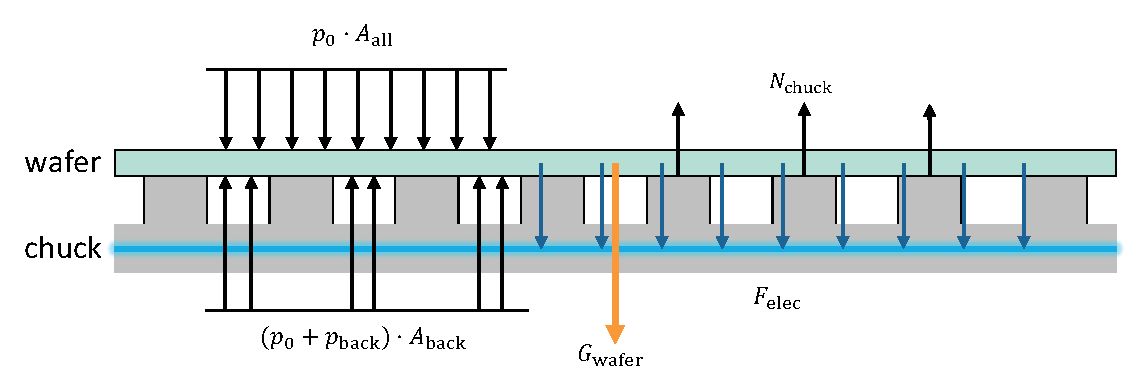
\includegraphics[width=1\linewidth]{principle/force__orig}
\caption[背吹平衡法晶圆受力]{背吹平衡法中晶圆受力分析图}
\label{fig:principle-backside-force}
\end{figure}

当静电卡盘处于正常工作状态时,晶圆牢固吸附在静电卡盘表面,其受力分析如图~\ref{fig:principle-backside-force},有:
\begin{equation}
\label{eq:principle-backside-force}
(p_{0} + p_{\mathrm{back}}) \cdot A_{\mathrm{back}} + N_{\mathrm{chuck}} = p_0 \cdot A_{\mathrm{all}} + G_{\mathrm{wafer}} + F_{\mathrm{elec}}
\end{equation}
其中:
\begin{itemize}
  \item $p_{0}$ : 环境压强(绝对)
  \item $p_{\mathrm{back}}$  : 背吹压强(相对于$p_{0}$)
  \item $A_{\mathrm{back}}$  : 晶圆背面气压等效作用面积(见\ref{principle-area})
  \item $A_{\mathrm{all}}$   : 晶圆总面积
  \item $N_{\mathrm{chuck}}$ : 静电卡盘表面向晶圆提供的总支持力
  \item $G_{\mathrm{wafer}}$ : 晶圆总重力
  \item $F_{\mathrm{elec}}$  : 晶圆所受总静电吸引力
\end{itemize}
当晶圆即将脱附时,有 $N_{\mathrm{chuck}} \to 0$ ;此时 \eqref{eq:principle-backside-force} 可近似为:
\begin{equation*}
\label{eq:principle-backside-force'}
(p_{0} + p_{\mathrm{back}}) \cdot A_{\mathrm{back}} = p_0 \cdot A_{\mathrm{all}} + G_{\mathrm{wafer}} + F_{\mathrm{elec}}
\end{equation*}
即:
\begin{equation}
\label{eq:principle-backside-force''}
F_{\mathrm{elec}} = (p_{0} + p_{\mathrm{back}}) \cdot A_{\mathrm{back}} - p_0 \cdot A_{\mathrm{all}} - G_{\mathrm{wafer}}
\end{equation}


\subsection{脱附条件}\label{sec:principle-backside-dechuck}

背吹平衡法需要\emph{制造}并\emph{检测}晶圆即将脱附至完全脱附的状态,从而间接获得静电力大小。制造脱附条件的基本方法是使背吹压力相对于静电吸引力更大,可通过提高气压、降低电压等方式实现(见 \ref{sec:priorArt-backside} )。检测脱附的方法主要是监测晶圆在脱附时产生变化的物理量,如位移/挠度、电极回路电流、背吹回路压强/流量等。 %TODO:analysis/xref



\section{试验环境}\label{sec:principle-env}

静电卡盘最常见的工作条件是在工艺腔室中,周围环境为真空,有时存在等离子体(单极型静电卡盘必须有等离子体存在才能产生静电吸引力)。已有方案大多选择同样在真空腔室中进行测量,甚至加入等离子体,以复现实际工艺条件。虽然这样可能有助于提高测试结果的准确度,但在真空与等离子体条件下试验存在如下问题:
\begin{itemize}
  \item 需要围绕选定的静电卡盘及试验用到的各种装置搭建专用真空腔室,其设计复杂,加工要求高;一旦更换被测静电卡盘型号,需重新设计腔室及配套系统;这部分的工作量与复杂程度甚至已经逼近刻蚀机的核心部分。
  \item 抽真空需使用真空泵,花费数小时才能达到真空,若需打开腔室进行调整,则需先平衡气压,再改动,再抽真空;费时费力。
  \item 真空下,背吹气体泄漏率较高 %TODO:xref/cite
  ,该流动过程可能对晶圆受力产生影响(见\ref{sec:principle-flow}节),使数据处理变得复杂。
  \item 有等离子体存在的时候,卡盘上方的空间基本无法放置任何测量装置(否则会遮挡等离子体,或与等离子体互相干扰),这为测量方案的设计带来了相当大的障碍。
\end{itemize}

因此,新方案将首先为大气环境设计,如可能,兼顾在真空条件下使用(原理不变,装置修改尽量小),但不考虑等离子体。



\section{背吹通道流动}\label{sec:principle-flow}

已有背吹平衡方案均假定晶圆背面受均匀压强作用,但未论证该假设的合理性 ---  即,背吹通道中存在的稳态流动是否会影响晶圆背面受力情况?若有,则测量方案的准确度可能会受到影响。因此,有必要分析晶圆背面的流动情况。


\subsection{建立CFD模型}\label{sec:principle-flow-cfd-setup}

为了方便后续仿真工作的开展,此处选择Comsol作为仿真软件;先搭建简化模型,做出基本判断,再根据后续试验需要,进一步添加细节,提高仿真准确度。

\begin{figure}[hbt]
\centering
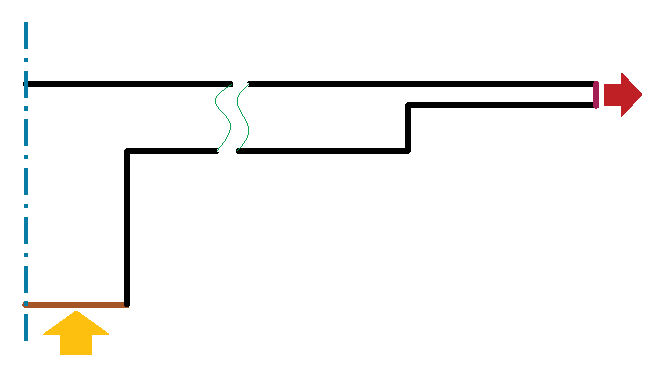
\includegraphics[width=0.72\linewidth]{principle/cfd__setup}
\caption[CFD建模示意]{Wafer背面流动CFD建模示意}
\label{fig:principle-flow-cfd-setup}
\end{figure}

根据静电卡盘几何尺寸,估计流动为充分发展的平板层流,选用\verb|spf|模块求解。几何模型选用\verb|2D Axisymmetric|(即旋转体),流道截面如图~\ref{fig:principle-flow-cfd-setup} 
\footnote{此处流道宽度由陶瓷介电层表面的凸台高度决定,但为了简化分析起见,暂时忽略凸台影响。}
;在正中间设一圆柱形进气口,直径\SI{1}{\mm},固定其压力为\SI{2}{\kPa}表压;在边缘处用均匀圆环形狭缝来等效晶圆与陶瓷介电层的接触密封,外侧设为出口,固定为大气压。

由于对实际接触密封情况不是很了解,设定参数扫描,求解狭缝宽度为\verb|10^{range(0,-1/2,-1)}[um]|,即1到\SI{0.1}{\micro\meter}对数等间隔时的流动情况。


\subsection{CFD仿真结果}\label{sec:principle-flow-cfd-result}

当狭缝宽度改变时,速度场变化不大,最大速度均出现在进口附近,之后速度迅速衰减至稳定,如图~\ref{fig:principle-flow-cfd-result-vel} 。

%TODO:动量呢?

在入口处对$v_z\ \rho$取面积分,得到质量流量如表\ref{tab:principle-flow-cfd-result-flow}。单位\si[per-mode=symbol]{\mg\per\minute}大致与sccm相当,即质量流量在狭缝宽\SI{1}{\micro\meter}时,仍低于1 sccm;狭缝变窄时,流量得非常快。这说明只要密封处的实际表面粗糙度足够低,接触足够紧密,则气体泄漏几乎可忽略不计;若安装流量计,则应选取较小量程的型号(一般为10 sccm)。

沿模型上边界(即晶圆下表面)绘制压强 -- 半径曲线,如图~\ref{fig:principle-flow-cfd-result-pressure} ,发现在流道中段压降满足$\Delta p \propto \log{r}$。 %TODO:derive by hand
当狭缝宽\SI{1}{\micro\meter}时,在中段存在明显压降(约\SI{0.6}{\kPa}),显然\textbf{不能忽略};但当狭缝更窄时,压降迅速衰减,当狭缝宽\SI{0.3}{\micro\meter}时已可忽略。当然,这是假定只有卡盘中央有一个气孔的时候的情形,而实际的静电卡盘为了控制温度分布均匀,在整个表面多处分布气孔,可使压强分布更均匀。即便如此,在处理实验数据时,应小心验证压强分布(可进一步构建三维流道模型以得到更准确的仿真数据),不能直接认为晶圆受均匀气压作用。

\begin{table*}[hbp]
\centering
\caption[CFD结果:质量流量]{CFD仿真结果:进口处质量流量}
\label{tab:principle-flow-cfd-result-flow}
\begin{tabular}{SS}
  \toprule[1.5pt]
  狭缝宽度/\si{\mm}  &  质量流量/\si{\mg\per\minute}  \\
  \midrule[1pt]
  \num{1.000}  &  \num{2.183e-1}  \\
  \num{0.316}  &  \num{9.628e-3}  \\
  \num{0.100}  &  \num{3.079e-4}  \\
  \bottomrule[1.5pt]
\end{tabular}
\end{table*}

\begin{figure}[hbp]
\centering
\includegraphics[width=0.72\linewidth]{principle/cfd__vel.png}
\caption[CFD结果:速度场]{CFD仿真结果:进口附近速度场}
\label{fig:principle-flow-cfd-result-vel}
\end{figure}

\begin{figure}[hbp]
\centering
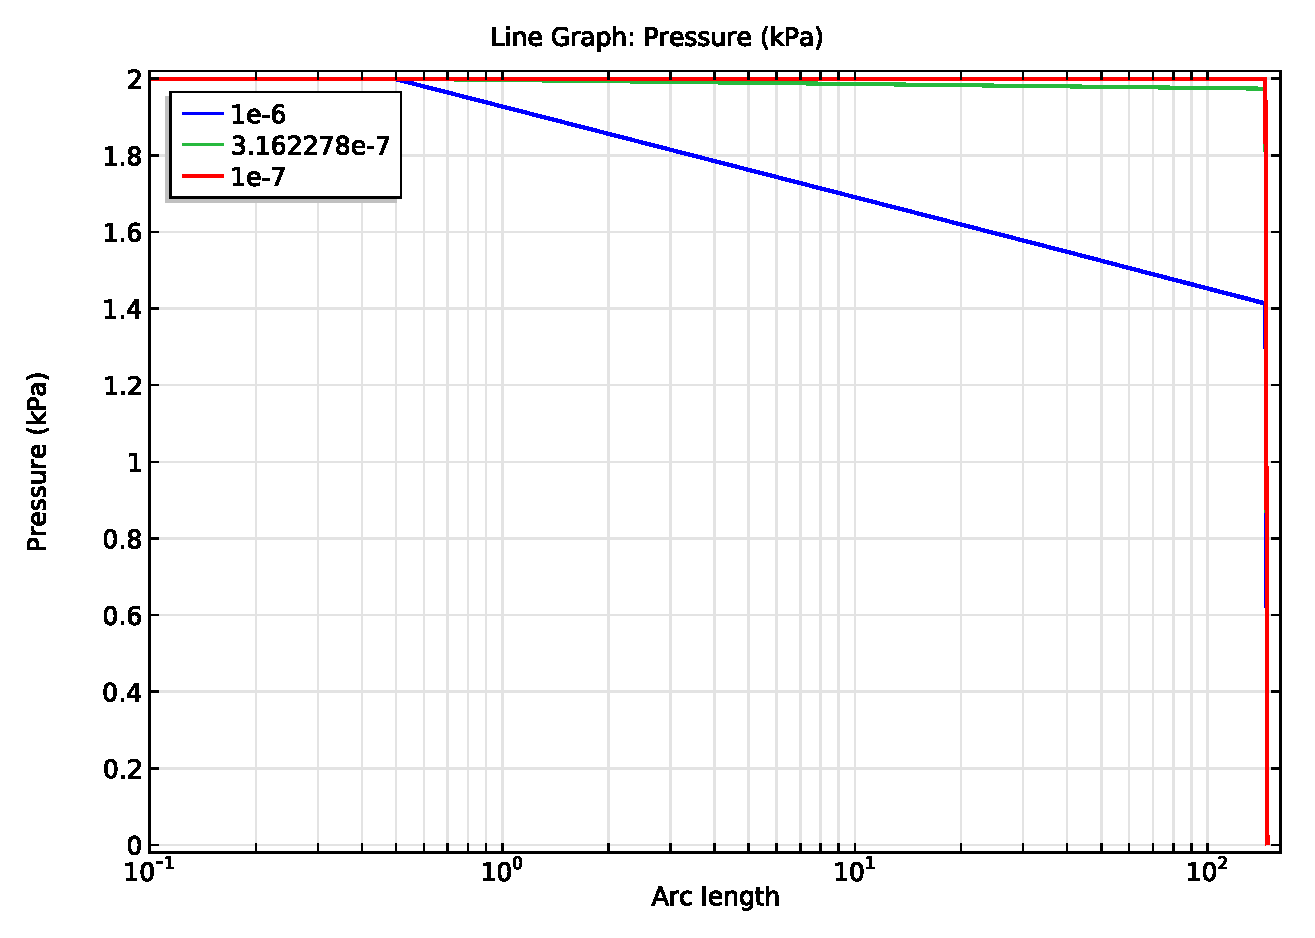
\includegraphics[width=1\linewidth]{principle/cfd__pressure}
\caption[CFD结果:压力分布]{CFD仿真结果:压力沿径向分布}
\label{fig:principle-flow-cfd-result-pressure}
\end{figure}

\clearpage



\section{间隙与部分脱附}\label{principle-gap}

已有脱附试验中(不限于背吹法)另一个共有问题:当\textbf{检测}到脱附时,晶圆实际已部分脱附,即脱附是一连续变化的过程  %TODO:cite 曹明路
;此时晶圆与卡盘的间隙大于未脱附(正常工作)时,而%TODO:xref bg equations
\begin{comment}
根据,
\end{comment}
静电力随着间隙扩大急剧下降,导致测得的静电力一定小于工作状态静电力,即测量存在较大系统误差。如能设法减小该误差,则可提高测量的准确度。

首先,虽然瞬态过程(如晶圆突然出现明显脱附等)容易检测,但此时晶圆并非处于平衡态(微观上可能已大部分脱附),且各种测量仪器均有不同程度的响应延迟(精度较高的仪器往往延迟也更大);这些因素均可产生系统误差。因此,应尽可能维持整个测量系统在准静态条件下。

然后,为了尽可能消除部分脱附的影响,希望能在整个脱附过程中尽可能早地检测到“脱附已开始”这一转折点;若此时间隙未明显扩大,则可认为静电力相对于工作状态偏差不大,系统误差减小。这需要选取合适的脱附特征物理量,并在尽量避免误判的同时,提高检测灵敏度。


\subsection{用微力探头减小间隙影响}\label{principle-gap-ruby}

\begin{figure}[tbhp]
\centering
\includegraphics[width=1\linewidth]{principle/gap__ruby__sch}
\caption{微力探头原理示意}
\label{fig:principle-gap-ruby-sch}
\end{figure}

如图~\ref{fig:principle-gap-ruby-sch} ,将一个三坐标测量机标准红宝石探头(图中以红色圆形表示,实际为球面),安装在微力传感器上,即组成一微力探头,可实时通过传感器监测探头受力;由牛顿第三定律,该力与微力探头施加在晶圆上的支持力$N_{\mathrm{probe}}$大小相等。在晶圆吸附后,使微力探头与已吸附的晶圆表面垂直接触,并确保$N_{\mathrm{probe}} \ll F_{\mathrm{elec}}$;当静电卡盘正常工作时,可认为$N_{\mathrm{probe}} \approx 0$。当晶圆开始脱附时,卡盘表面不再向晶圆提供支持力,即$N_{\mathrm{chuck}} \to 0$,而逐渐转由探头向晶圆提供支持力,即$N_{\mathrm{probe}}$逐渐增加。由于力传感器自身具有一定弹性,在此期间容许晶圆有一定的挠度,但由于$N_{\mathrm{probe}}$绝对数值较小,可以保证晶圆至少在与探头接触的一点处,与卡盘的间隙在一确定范围内,且该范围由传感器参数决定。因此,通过使用微力探头,可以在控制间隙的同时,有效判定晶圆是否已经脱附或部分脱附。

%TODO:introduce F-p curve schematic (or later?)



\section{压强等效作用面积}\label{principle-area}

气压平衡法中,另一个不确定度的来源是晶圆背面气压等效作用面积,即\eqref{eq:principle-backside-force}中的$A_{\mathrm{back}}$。
%TODO:cite nagoya
由于陶瓷介电层上的凸台高度较低(约\SI{10}{\micro\meter})与晶圆背面接触情况不明,尚不能直接断言$A_{\mathrm{back}}$等于晶圆背面所有未与陶瓷层凸台/边缘接触部分的面积。由于此处无法用普通CFD求解,需要设计额外的标定步骤,测出$A_{\mathrm{back}}$数值。


\subsection{自重平衡法}\label{sec:principle-area-gravity}

\begin{figure}[tbhp]
\centering
\includegraphics[width=1\linewidth]{principle/area__gravity__sch}
\caption[自重法测等效面积示意]{利用自重平衡法测量压强等效作用面积示意}
\label{fig:principle-area-gravity-sch}
\end{figure}

一种可行的测量方法如图~\ref{fig:principle-area-gravity-sch}。注意到在晶圆受力平衡关系中,只有重力的方向是任意的,其他力相对于卡盘坐标系的方向均固定。若将整个系统上下倒转\ang{180},则相当于只有重力的方向发生变化,进而将压强与已知大小的力建立对应关系,得到等效面积大小。

具体方法:分别在试验台正放和倒放两种状态下,加相同电压,完成背吹平衡试验,得到即将脱附时的背吹压强分别为$p_{\mathrm{back},1}$和$p_{\mathrm{back},2}$(可分别多做几组,取平均值,以减小随机误差干扰)。根据受力平衡关系有:
\begin{equation}
\label{eq:principle-area-gravity-orig}
\begin{aligned}
(p_{0} + p_{\mathrm{back},1}) \cdot A_{\mathrm{back}} & = p_0 \cdot A_{\mathrm{all}} + G_{\mathrm{wafer}} + F_{\mathrm{elec}} \\
(p_{0} + p_{\mathrm{back},2}) \cdot A_{\mathrm{back}} & = p_0 \cdot A_{\mathrm{all}} - G_{\mathrm{wafer}} + F_{\mathrm{elec}}
\end{aligned}
\end{equation}
两式相减:
\[
(p_{\mathrm{back},1} - p_{\mathrm{back},2}) \cdot A_{\mathrm{back}} = 2 G_{\mathrm{wafer}}
\]
即:
\begin{equation}
\label{eq:principle-area-gravity-derived}
A_{\mathrm{back}} = \frac{2 G_{\mathrm{wafer}}}{p_{\mathrm{back},1} - p_{\mathrm{back},2}}
\end{equation}
即求得$A_{\mathrm{back}}$数值。需要注意的是,$A_{\mathrm{back}}$可能与所加电压、晶圆材料、厚度等各种参数相关,需改变条件,多次试验,求出$A_{\mathrm{back}}$对各参数的敏感度。




%TODO:summarize what's included in the actual experiment
\section{本章小结}\label{sec:principle-summary}

%% !TeX root = ../main.tex
\chapter{测量平台设计与搭建}



\section{总体设计}\label{sec:rig-overall}

根据上文规划的测量方案以及实际需求,设计大气环境下的静电卡盘静电力检测平台,希望能达成如下目标:

\begin{enumerate}
  \item 实现用背吹平衡 -- 微力探头法检测静电力
  \item 自动化检测过程,减小人为误差
  \item 采集检测过程中各关键变量,方便后续数据处理与分析
\end{enumerate}

下面将详细阐述测量平台的设计方案。


\subsection{测量平台组成}\label{sec:rig-overall-comp}

\begin{figure}[tbh]
\centering
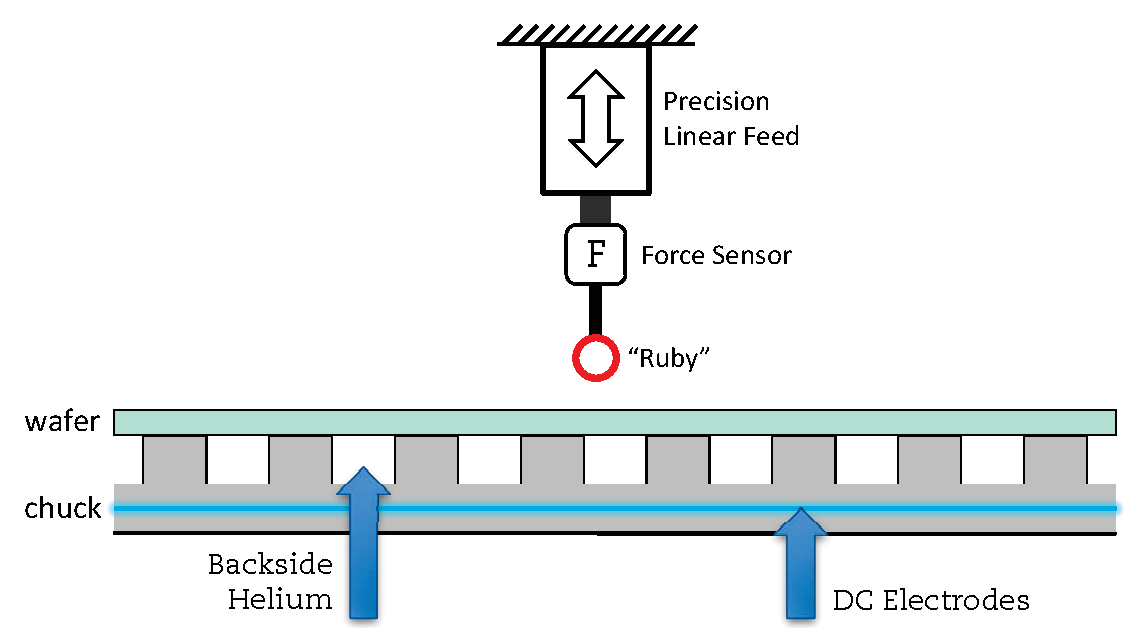
\includegraphics[width=1\linewidth]{rig/overall__sch}
\caption{测量平台总体设计示意}
\label{fig:rig-overall-sch}
\end{figure}

如图~\ref{fig:rig-overall-sch},整个测量平台由以下组件构成:

\begin{itemize}
  \item 待测静电卡盘及其配套静电电源
  \item 微力探头组件
  \item 背吹控制系统
  \item 机械结构
  \item 电控与数据采集系统
\end{itemize}

除静电卡盘与电源外,其他组件均需自行设计、搭建。


\subsection{检测流程}\label{sec:rig-overall-proc}

一次完整的检测过程分如下步骤完成:

\begin{enumerate}
  \item 准备静电卡盘
  \begin{enumerate}
    \item 用无水乙醇擦拭静电卡盘与晶圆
    \item 将晶圆小心地放置在静电卡盘陶瓷层正中央
    \item 开启静电电源,调节电极电压至目标电压
  \end{enumerate}
  
  \item 准备测量平台
  \begin{enumerate}
    \item 降下微力探头,使其轻轻接触晶圆
    \item 确认背吹控制系统中调压装置均处于零位
  \end{enumerate}
  
  \item 检测
  \begin{enumerate}
    \item 开始自动记录微力探头受力、背吹入口气压两变量
    \item 背吹气压接通并缓慢、均匀地上升
    \item 当微力探头受力即将达到其满量程时,自动切断背吹气压,检测停止
  \end{enumerate}
  
  \item 后续处理
  \begin{enumerate}
    \item 导出采集到的数据
    \item 微力探头复位上升
    \item 切断静电电源,短接两电极引线,消除部分残余电荷
    \item 小心将晶圆取下
  \end{enumerate}
\end{enumerate}



\clearpage



\section{微力探头组件设计}\label{sec:rig-probe}

图~\ref{fig:rig-overall-sch}中,卡盘上方的组件即为微力探头组件微力探头组件,其在\ref{principle-gap-ruby}节中提到的微力传感器和红宝石探头的基础上,增设精密直线进给机构:固定端连接在框架上,移动端与力传感器的固定端相连,用于驱动探头沿z方向移动,以实现“轻轻接触晶圆”这一动作。


\subsection{微力传感器选型}\label{sec:rig-probe-sensor}

微力传感器是探头组件中的核心元件,因此优先选型。考虑到其在测量系统中的作用,主要关心以下参数:

\begin{enumerate}
  \item \textbf{量程}:
    无论在轻触阶段还是在脱附检测阶段,探头均不应向晶圆施加过大的力。粗估静电力处于$\SI{10}{\newton}$至$\SI{200}{\newton}$之间,探头施加的力应低于其$1 ~\%$,即微力传感器应能准确测量 大致在$\SI{0.1}{\newton}$至$\SI{2}{\newton}$范围内的单轴压缩力。
  \item \textbf{分辨力}:
    微力传感器需能检测到微小的受力变化,根据上述关于量程的讨论,应能至少分辨出$\SI{1}{\milli\newton}$的力增量。不同的传感器可能对分辨力的标称方法不同,应结合其输出信号特点,判定其是否满足要求。
  \item \textbf{刚度}:
    微力传感器的敏感端存在一位移,一般服从胡克定律,与受力成比例关系。\ref{principle-gap}节中讨论了晶圆与卡盘间气隙可能对静电力产生的影响。若传感器刚度较高,则可更好地控制气隙大小,并在气隙明显扩大之前检测出脱附;但另一方面,高刚度使轻触晶圆更难实现(见\ref{sec:rig-probe-feeding}节\eqref{eq:rig-probe-feeding-vel}式)。因此该参数并无明确要求,仅做为选型时的参考。
  \item \textbf{过载能力}:
    考虑到在安装、调试过程中,以及硅晶圆突然完全脱附时,探头均可能瞬间受到较大的力的作用;若微力传感器承受过载能力较好,则可避免其意外受损。
\end{enumerate}

初步筛选市面上各种微力传感器得到表~\ref{tab:rig-probe-sensor}。若考虑量程、精度、分辨力,1050V1较差;若考虑刚度,LSB200较差;若考虑过载性能,FT-S10000较差。由上文讨论,量程、分辨力是最重要的性能指标,而刚度因素较为次要,且即使是刚度最低的LSB200,其值也已达到$\SI[per-mode=symbol]{1}{\milli\newton\per\micro\meter}$,因此选择LSB200型应变式微力传感器。

% generated using http://www.tablesgenerator.com/latex_tables
\begin{table}[htbp]
\begin{minipage}{1\linewidth}
\centering
\caption{微力传感器选型表}
\label{tab:rig-probe-sensor}
\begin{tabular}{@{}lllccc@{}}
\toprule[1.5pt]
生产商 &  &  & Futek & Dytran & FemtoTech \\
型号 &  &  & LSB200 & 1050V1 & FT-S10000 \\
\midrule[1pt]
原理 &  &  & 应变式 & 压电式 & MEMS \\
输出信号 & 类型 &  & 电阻电桥 & 电压 & 电压 \\
 & 单位 &  & $\si[per-mode=symbol]{\milli\volt\per\volt}$ & V & V \\
灵敏度 & 满量程 & 输出 & 0.5 & 5 & 2 \\
 & 单位受力 & 输出/$\si{\newton}$ & 5.0E+00 & 1.1E-01 & 2.0E+02 \\
分辨力 &  & $\si{\micro\newton}$ & --\footnote{未标称,下同} & 600 & 0.5 \\
刚度 &  & $\si[per-mode=symbol]{\newton\per\micro\meter}$ & 0.001 & 1996.45 & -- \\
\midrule[1pt]
满量程 & 拉(+) & $\si{\newton}$ & 0.1 & 44.48 & 0.01 \\
 & 压(-) & $\si{\newton}$ & 0.1 & 44.48 & 0.01 \\
最大载荷 & 拉(+) & $\si{\newton}$ & 1 & 889.64 & 0.03 \\
 & 压(-) & $\si{\newton}$ & 1 & 889.64 & 0.03 \\
\midrule[1pt]
线性度 &  & \% FS & 0.1 & 1 & \multirow{2}{*}{--} \\
 &  & $\si{\newton}$ & 2.00E-04 & 8.90E-01 &  \\
滞回 &  & \% FS & 0.1 & \multirow{2}{*}{--} & \multirow{2}{*}{--} \\
 &  & $\si{\newton}$ & 2.00E-04 &  &  \\
重复精度 &  & \% FS & 0.05 & \multirow{2}{*}{--} & \multirow{2}{*}{--} \\
 &  & $\si{\newton}$ & 1.00E-04 &  &  \\
\bottomrule[1.5pt]
\end{tabular}
\end{minipage}
\end{table}


\subsection{进给机构选型}\label{sec:rig-probe-feeding}

进给机构的主要作用为完成“轻触晶圆”动作,其移动组件可为推杆或直线滑移台(优先推杆),驱动方式可为手动或电动(优先电动)。对于手动进给机构,只需考虑其最小步长(受静摩擦等因素限制),因此下面主要讨论电动进给机构的选型。主要关心以下参数:

\begin{enumerate}
  \item \textbf{低速性能}:
    由于当探头接触到晶圆时,接触力会突增,为了限制接触力,需要控制探头以较低速度接近晶圆,直至微力传感器读数出现明显变化,即命令进给机构停止运动。这要求进给机构能够在低速下平稳运行,即低速速度波动较小,或爬行现象不明显。参考运动速度可按\eqref{eq:rig-probe-feeding-vel}计算:
    \begin{equation}
    \label{eq:rig-probe-feeding-vel}
    v_{\mathrm{ref}} = \frac{ F_{\mathrm{thres}} }
                            { k_{\mathrm{sensor}} \cdot t_{\mathrm{delay}} }
    \end{equation}
    其中:
    \begin{itemize}
      \item $F_{\mathrm{thres}}$  : 探头接触晶圆时最大允许施加的力
      \item $k_{\mathrm{sensor}}$ : 微力传感器刚度
      \item $t_{\mathrm{delay}}$  :  从探头受力跳变到进给机构停止运动的总时滞(包括机械惯性、信号传输延迟等)
    \end{itemize}
    代入LSB200相关数据(
    $F_{\mathrm{thres}} = \SI{1}{\milli\newton}$,
    $k_{\mathrm{sensor}} = \SI[per-mode=symbol]{0.001}{\newton\per\micro\meter}$
    ),在$t_{\mathrm{delay}} = \SI{0.01}{\second}$时计算参考速度为$\SI[per-mode=symbol]{100}{\micro\meter\per\second}$。
  \item \textbf{总行程}:
    小型精密电动进给机构行程较低,可采用粗精二级调节的方法:先用手动或电动方式粗调整个微力探头组件,将其固定在接近晶圆的位置上,再驱动精密进给机构完成轻触动作。为了方便粗调,希望总行程至少为$\SI{5}{\milli\meter}$。
  \item \textbf{背隙/回差/抖动}:
    完成轻触晶圆动作后,进给机构需保持原位不动(锁定),因此对于能够自锁的机构,不应有回差影响;对于不能自锁的机构,需确认其因反馈控制产生的抖动在合理范围内。
\end{enumerate}

由于候选型号较多,完整的选型表参见附录B。 %TODO:xref appendix
最终选定的电动进给机构为LAC10A-T4精密电动推杆,其原理为步进电机驱动滚珠丝杠,有效行程$\SI{10}{\milli\meter}$,重复定位精度$\pm\SI{1.5}{\micro\meter}$,具有自锁特性。



\clearpage



\section{背吹控制系统设计}\label{sec:rig-pressure}

背吹平衡法需要控制静电卡盘背吹入口压强\footnotemark{}缓慢、平稳上升,并实时测量、记录该压强数值;最好还能同时测出进入背吹通道的流量。显然,整个系统可分为供压与传感两部分,关键参数为压强、流量。
%TODO:cite力大小来源,最好北方微电子
按照待测静电卡盘的参数($d = \SI{296}{\milli\meter}$,$F \leq \SI{200}{\newton}$,压强等效面积定为 总面积$1/2$)估算,背吹入口压强最大不会超过$\SI{6}{\kilo\pascal}$。由于之前尚未有在大气环境下针对类似尺寸的静电卡盘的背吹试验,流量范围未知,需通过实测获得。

\footnotetext{由于测量平台处于大气环境下,所有压强均为表压(相对于大气压强),下略。}


\subsection{供压方案分析}\label{sec:rig-pressure-supply}

常见的气压控制元件主要应用于气动机械(如气缸、气爪、气动回转台等),压强下限一般为$\SI{0.1}{\mega\pascal}$级,与系统要求差距很大,因此需仔细拟定气压控制方案,选择合适的组件保证气压精确控制。

\subsubsection{集成电子压强控制单元}\label{sec:rig-pressure-supply-integrated}

这类产品集成了压强控制所需的所有电、气元件,接受一个电信号输入作为压强设定点,控制出口压强等于该设定点。其中,部分产品包括完整的显示、操作单元、通信接口等,如WIKA CPC2000/CPC6000压强控制器等(图~);部分产品只有简单的指示器,设定点为模拟信号(如$\num{4} \sim \SI{20}{\milli\ampere}$信号),如TESCOM ER3000/ER5000系列、SMC ITV00x0系列电子比例阀等。完整的压强控制器较为昂贵,但精度较高,量程可选余地较大;电子比例阀成本较低,但其量程一般仍为气动机械级,而其小量程型号允许的流量过低(如SMC ITV0010型,最低输出压强$\SI{1}{\kilo\pascal}$,最大流量仅$\SI[per-mode=symbol]{3.5}{\liter\per\minute}$)。

\begin{figure}[tbh]
\centering
\includegraphics[width=0.75\linewidth]{rig/pressure__supply__cpc6000.png}
\caption{WIKA CPC6000压强控制器}
\label{fig:rig-pressure-supply-cpc6000}
\end{figure}

\subsubsection{反馈控制微型气泵}\label{sec:rig-pressure-supply-pump}

参考CPC2000的工作原理示意图(图~\ref{fig:rig-pressure-supply-cpc2000-sch}),可用独立元件设计类似的压强控制系统,如图~\ref{fig:rig-pressure-supply-pump-sch}:使用直流电机驱动的微型气泵作为压力源,压强变送器提供反馈信号,闭环PI控制气泵输出功率。为减小气泵固有的压强波动,可采取如下措施:

\begin{enumerate}
  \item 在泵与背吹通道入口间增设双端气瓶,通过增加惯性环节的方式降低压强波动;
  \item 在背吹通道入口处加设一节流阀通向大气,避免电机反复启停造成的压强波动;
\end{enumerate}

\begin{figure}[tbh]
\centering
\includegraphics[width=1\linewidth]{rig/pressure__supply__cpc2000__sch.png}
\caption{CPC2000工作原理示意}
\label{fig:rig-pressure-supply-cpc2000-sch}
\end{figure}

\begin{figure}[tbh]
\centering
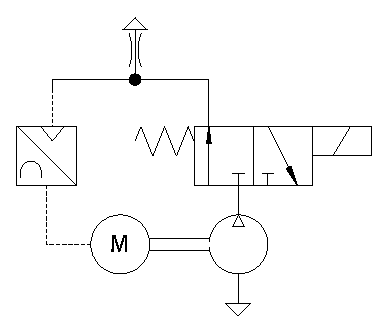
\includegraphics[width=0.618\linewidth]{rig/pressure__supply__pump__sch}
\caption{反馈控制微型气泵示意}
\label{fig:rig-pressure-supply-pump-sch}
\end{figure}

\subsubsection{精密机械式减压阀}\label{sec:rig-pressure-supply-reg}

机械式减压阀的原理是通过膜片平衡,反馈控制小孔开度,从而达到稳定输出压强的目的。即便是原本应用于气动机械的精密减压阀,根据其原理不同,有些产品允许出口压强低于其标称最低输出压强,只不过此时输出压强随流量改变。如SMC IR1000型精密减压阀(图~\ref{fig:rig-pressure-supply-ir1000}),标称调压范围$\num{5} \sim \SI{200}{\kilo\pascal}$,标称灵敏度$\SI{0.4}{\kilo\pascal}$。除了可用作电子比例阀的前置减压阀外,有可能直接接入背吹通道,作为小开度节流阀使用,提供$\num{0} \sim \SI{5}{\kilo\pascal}$范围内的缓慢变化的压强。
%TODO:xref rig test and indicate

\begin{figure}[tbh]
\centering
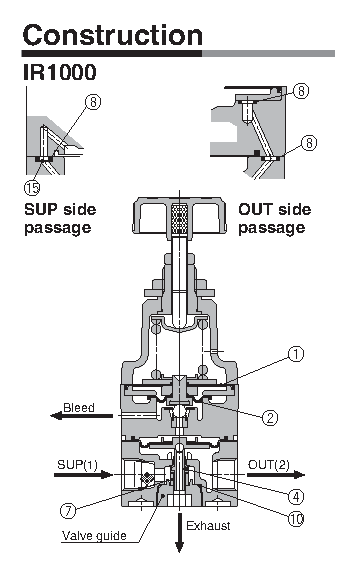
\includegraphics[height=0.9\textheight]{rig/pressure__supply__IR1000}
\caption{IR1000简化剖视}
\label{fig:rig-pressure-supply-ir1000}
\end{figure}


\subsection{传感部分选型}

无论供压部分采用何种方案,均不影响压强传感器的选型。完整的选型表见附录B。 %TODO:xref appendix
最终选定Honeywell STD720精密差压变送器(量程可在$\pm \num{1} \sim \pm \SI{100}{\kilo\pascal}$范围内任意配置,基础准确度$0.05\%$,输出$\num{4} \sim \SI{20}{\milli\ampere}$模拟信号、HART现场总线协议)。另外配置$\SI{16}{\kilo\pascal}$量程的机械指针式压强计,辅助调试。



\clearpage



\section{机械结构设计}\label{sec:rig-model}

根据图~\ref{fig:rig-overall-sch},设计测试平台的机械结构。为了方便加工、搭建,选用标准$\num{30} \times \SI{30}{\milli\meter}$系列开槽铝合金型材及配套标准连接件,与依据待测静电卡盘的外形尺寸设计的连接板共同构成框架结构;其他组件均通过连接件与之相连。框架结构的简化三维模型如图~\ref{fig:rig-model-all-iso}\footnote{型材连接部分零件数较多,因此并未全部在总装配体三维模型中表示出。}。

\begin{figure}[p]
\centering
\includegraphics[width=1\textwidth]{rig/model__all__iso.png}
\caption{测试平台装配体三维模型}
\label{fig:rig-model-all-iso}
\end{figure}


\subsection{静电卡盘连接板}\label{sec:rig-model-base}

该连接板位于整个测试平台中心,其尺寸与配合特征主要由静电卡盘决定,并间接决定了整个框架的尺寸。静电卡盘通过螺钉紧固在连接板上,因此连接板需提供相配合的螺纹孔与承载面。如图~\ref{fig:rig-model-echuck-back}\footnotemark{},静电卡盘的底部有多个功能特征,除氦气背吹接口需特殊设计外,其他特征(如直流电极接口、顶针孔等)均需裸露在外以正常使用,因此连接板上对应位置开槽。氦气背吹接口并未采用常见的螺纹连接方式,而是一$\diameter{}4$光孔,需设计密封接头与之相连。如图~\ref{fig:rig-model-echuck-plug-assy},用三个紧定螺钉使密封接头上表面与卡盘背面紧密配合,通过标准O型圈形成端面密封,其另一端提供M5内螺纹,与标准气动快装接头连接,方便配管。

\footnotetext{北方微电子公司内部图纸,仅保留轮廓与功能描述。}

\begin{figure}[tbhp]
\centering
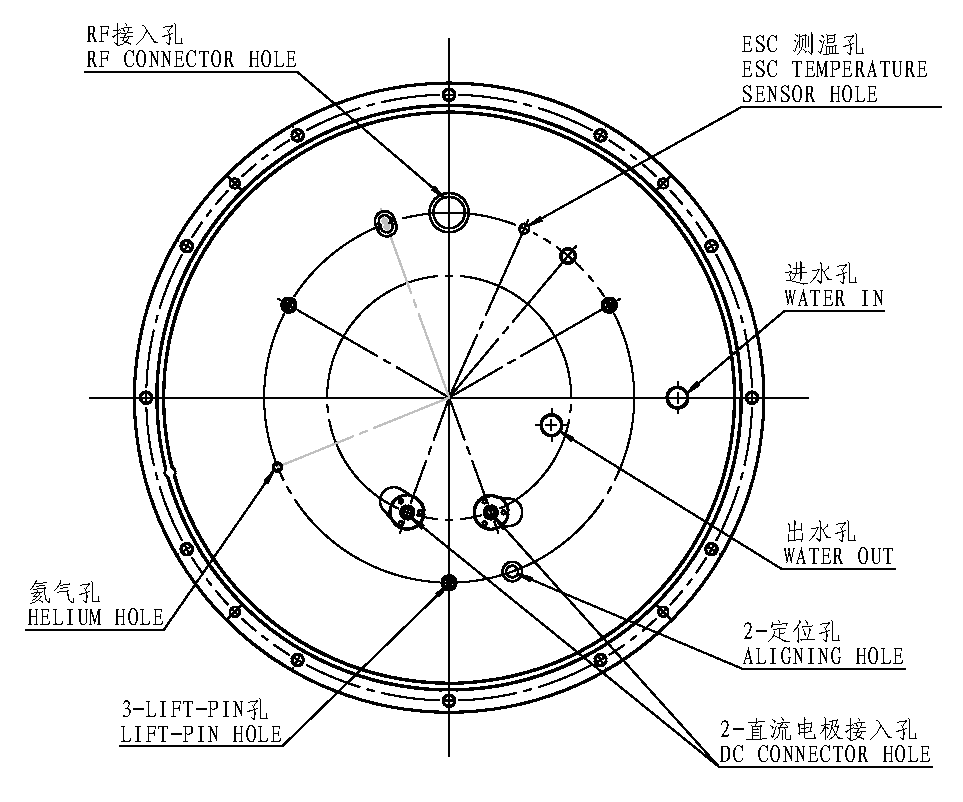
\includegraphics[height=0.45\textheight]{rig/model__echuck__back}
\caption{静电卡盘背面特征工程图}
\label{fig:rig-model-echuck-back}
\end{figure}

\begin{figure}[tbhp]
\centering
\includegraphics[height=0.45\textheight]{rig/model__echuck__plug__assy2}
\caption{端面密封设计工程图}
\label{fig:rig-model-echuck-plug-assy}
\end{figure}


\subsection{型材框架结构}\label{sec:rig-model-frame}

框架主体为三层对称结构:中间一层是静电卡盘连接板,上下各用4根型材连接成正方形(型材间使用铸钢角件和紧定螺钉连接);层与层之间用4根纵向型材负责承重,在连接板侧使用$\num{50}\times\num{50}\times\SI{30}{\milli\meter}$挤压角件连接(三维模型中已表示出),在正方形型材侧使用$\num{60}\times\num{60}\times\SI{30}{\milli\meter}$角件连接。这种连接方式的主要优点是不依靠型材与角件的摩擦力承受重量,而是靠型材、角件、连接螺栓将载荷传至地面。

框架主体以外,还有2根型材组成的简易手动定位结构,用于连接微力探头,其横梁通过T型螺母、普通螺栓、大垫圈紧固在最上层正方形的下侧,竖梁使用$\num{60}\times\num{60}\times\SI{30}{\milli\meter}$角件连接在横梁上。通过改变这2根型材连接位置,即可改变微力探头在晶圆平面上的投影位置。


\subsection{微力探头装配}\label{sec:rig-model-probe}

%TODO:refine description -- in more detail

如图~\ref{fig:rig-model-probe},设计连接板,将微力探头组件\footnotemark{}通过沉头螺钉固定在其上;若选择使用电动推杆,需先使用自带的六角薄螺母固定在图示连接块上。连接板后部设导向键,配合T型螺母、内六角螺栓连接在型材上。

由于此处空间较小,还有较为敏感的微力传感器(最大承受$\SI{1}{\newton}$力),应特别注意装配顺序:

\begin{enumerate}
  \item
    传感器处于平放状态(贴有商标一面向上),轻轻握住传感器活动端,小心将红宝石探头(需加M2$\to$M3转接头)旋入、拧紧;
  \item
    使手动平移台/电动推杆处于伸长状态,轻轻握住传感器固定端,将其连接在平移台/推杆上。
  \item
    手持平移台/推杆,将其通过沉头螺钉固定在连接板上。
\end{enumerate}

\footnotetext{三维模型中两组微力探头是为了同时在图中表示手动和电动两种情况下的连接方式,实际仅选装一组。}

\begin{figure}[tbhp]
\centering
\includegraphics[height=0.45\textheight]{rig/model__probe.png}
\caption{探头组件数字模型}
\label{fig:rig-model-probe}
\end{figure}



\clearpage



\section{电控与数据采集系统设计}\label{sec:rig-ctrl}

为了实现检测过程自动化,减小人操作对结果产生的干扰,设计电控与数据采集系统。检测平台中所有电子模块及其信号流动关系如图~\ref{fig:rig-ctrl-sch}。

\begin{figure}[tbhp]
\centering
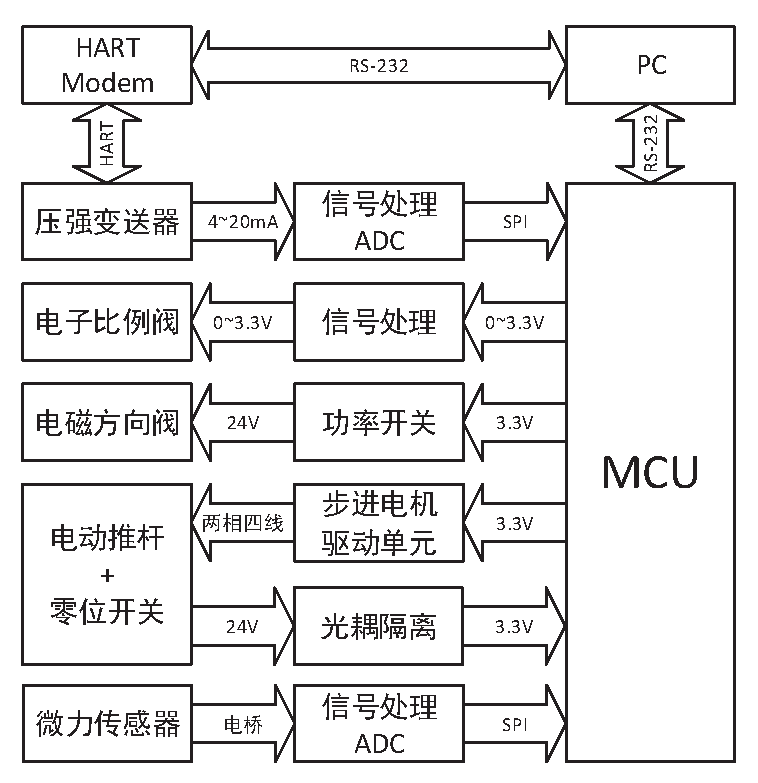
\includegraphics[height=0.5\textheight]{rig/ctrl__sch}
\caption[电控系统框图]{电控与数据采集系统模块框图}
\label{fig:rig-ctrl-sch}
\end{figure}




\section{搭建与调试}\label{sec:rig-build}
%% !TeX root = ../main.tex
\chapter{检测平台搭建与调试}\label{ch:impl}







%-------------------------------------------------------
%                       stash
%-------------------------------------------------------


由于LSB200微力传感器安全过载仅\SI{1}{\newton},装配时应特别小心,避免对其造成不可恢复的损伤。正确的装配方法如下:

\begin{enumerate}
  \item
    将LSB200接入电控系统
    %TODO:xref AD7730
    ,并在整个装配过程中监测其读数,尽量避免其受力超过满量程。
  \item
    LSB200处于平放状态(贴有商标一面向上),轻轻握住LSB200活动端,将螺纹转接头的M3外螺纹端旋入LSB200活动端,并在保证LSB200不过载的同时,将转接头旋紧。
  \item
    用小钳子夹住转接头,将红宝石探头旋入转接头的M2内螺纹端。
  \item
    使LAC-10A/JYPY-02213处于伸长状态,轻轻握住传感器侧面(固定端),将其连接在推杆末端/平移台上。
  \item
    将LAC-10A/JYPY-02213固定在连接板上。
\end{enumerate}


由于检测平台处于试验阶段,电控系统组成随时可能发生变化,因此直接使用最小系统版作为MCU载体。
%% !TeX root = ../main.tex
\cleardoublepage
\chapter{试验与数据处理}\label{ch:exp}

前面两章中设计并搭建出了静电卡盘静电力检测平台。为验证该平台确实能有效检测静电力,本章中重点讨论在该平台上进行的静电力检测试验。由于检测平台的组成、工作条件、检测原理均与已有的检测系统存在差异,需先通过前期试验逐步确定合理的检测流程,解决或回避检测中可能出现的问题,并验证检测原理与检测平台设计方案可行后,设计正式试验,获取并处理待测静电卡盘在不同条件下的静电力检测数据,为进一步分析提供基础。



\section{前期试验}\label{sec:exp-pilot}


\subsection{检测流程}\label{sec:exp-pilot-proc}

整个检测流程可分为三个阶段:准备过程、加压检测、以及后续处理。准备工作包含如下步骤:首先将晶圆放置在静电卡盘上,然后接通静电电源,施加目标静电电压,等待晶圆完全吸附;之后,启动电控系统,控制微力探头与晶圆接触,即准备完成。图~\ref{fig:exp-touchdown}~为此时检测平台的状态:由于此时电磁阀尚未接通,背吹通道压强为0,电极作用于晶圆的静电力与介电层表面对晶圆的支持力平衡,而微力探头只向晶圆施加一微小的力(约\SI{10}{\mN},见\ref{sec:impl-pcb-probe}节)。在确认机械减压阀处于零位后,即可开始加压检测:电控系统在开启电磁阀的同时开始采集背吹压强与探头受力数据,并将其实时发送到PC端;之后,手动操作减压阀旋钮,缓慢、均匀地增加其开度,背吹压强随之逐渐增加,直至探头受力超过其满量程的一定比例(暂定为80\%),电控系统自动切断电磁阀并停止采集数据。之后需要做的后续处理工作主要包括:PC端保存数据、切断静电电压、微力探头回零、移除晶圆等。

为提高可重复性,尽量保持两次检测间独立,每次检测完成后,均将静电卡盘电极短接一段时间,再移除晶圆,以减小介电层与晶圆表面残余电荷产生的残余吸附力影响。由于前期试验的主要目的是验证原理与平台设计的可行性,静电卡盘电极电压取的间隔可以较大,以便定性观察电压对静电力的影响。

\begin{figure}[p]
\centering
\includegraphics
  [max size={1\linewidth}{0.9\textheight}]
  {exp/touchdown.jpg}
\caption{检测平台与吸附的硅晶圆(加压前)}
\label{fig:exp-touchdown}
\end{figure}


\subsection{主要问题及解决思路}\label{sec:exp-pilot-fix}

前期试验过程中,发现了若干可能影响检测准确性与可重复性的问题,以下将一一说明并提出解决思路。

\subsubsection{减压阀输出压强尖峰}\label{sec:exp-pilot-fix-overshoot}

由于在检测过程中要求减压阀工作压强低于其保压下限,其压强与阀开度关系存在明显非线性,尤其是输出压强刚刚超过0时,会在短时间内突变,甚至产生一个高达\SI{0.4}{\kPa}的尖峰,如图~\ref{fig:exp-overshoot-before}~所示压强 -- 时间曲线。当尖峰出现时,晶圆受到一个瞬间冲击,有可能发生提前脱附现象,从而影响检测结果准确性。经反复试验发现,由于压强与机械减压阀的小孔开度相关(见\ref{sec:rig-pressure-supply-reg}节),当开度在零点附近时,开度调节膜片位置稍稍变化即可导致出口处压强迅速上升,之后膜片才起到反馈作用,压强稍微回落一点。为了消除这个过冲,可改进操作机械减压阀的方法如下:在阀开度即将达到零点时,不再直接旋转减压阀旋钮,改为用手指轻轻触碰旋钮,对其施加一个微小的扭矩;该扭矩在减压阀内部被转化为施加在膜片上的一个微小的力,使小孔开度微量增加,即可减小压强尖峰的高度;等初始跳变结束后,可恢复慢速旋转减压阀旋钮以控制压强缓慢上升。图~\ref{fig:exp-overshoot-after}所示的压强 -- 时间曲线即为采用了改进的操作方法后得到的典型的压强 -- 时间曲线(部分),其中压强跳变阶段无过冲,且拐点约为\SI{0.2}{\kPa},说明改进的操作方法可有效抑制尖峰,使压强变化更平缓。

\begin{figure}[tbhp]
  \centering
  \begin{subfigure}{1\textwidth}
    \centering
    \includegraphics[width={0.7\textwidth}]{exp/overshoot}
    \caption{原有较大尖峰}
    \label{fig:exp-overshoot-before}
  \end{subfigure}
  \par\bigskip
  \begin{subfigure}{1\textwidth}
    \centering
    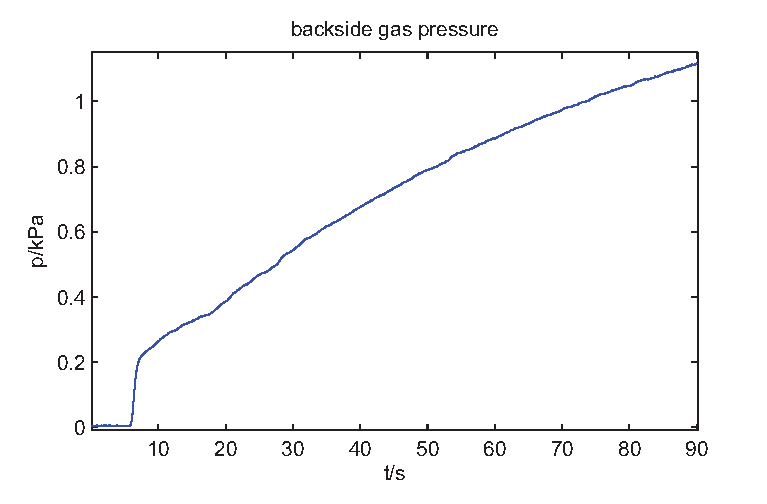
\includegraphics[width={0.7\textwidth}]{exp/overshoot-fix}
    \caption{改进操作方法后尖峰消失}
    \label{fig:exp-overshoot-after}
  \end{subfigure}
  \caption{减压阀输出压强尖峰}
  \label{fig:exp-overshoot}
\end{figure}

\subsubsection{晶圆颗粒污染与放置}\label{sec:exp-pilot-fix-wafer}

前期试验后发现,即使在同一电压下,测得的晶圆脱附压强仍有较大散布,推测该随机误差并非检测原理产生,而是每一次检测时,由于各种因素影响,难以做到晶圆吸附条件完全相同,由此导致晶圆所受静电力大小与分布自然存在差异,引起脱附压强较大散布。由静电卡盘工作原理知,晶圆与介电层间存在的颗粒污染对静电力有较大影响,考虑到检测平台处于大气条件下,且前期试验未能在超净间中进行,该因素可能是造成压强散布的主要因素之一。为了尽可能消除颗粒污染影响,可在每次试验前,先使用无纺布蘸无水乙醇擦拭晶圆,等无水乙醇挥发后,再将晶圆放置于静电卡盘上,加电吸附。另一个可能的影响因素是晶圆放置的位置。由于晶圆是手动放置在静电卡盘上的,并不能保证每次其圆心都与静电卡盘圆心重合,总是存在一定误差;当偏心过大时,可能会发生晶圆已完全气浮时,微力探头示数仍无明显变化的情况,导致无法根据微力探头数据准确判定脱附时刻。解决方法是每次在放置晶圆后,反复肉眼观察并调整晶圆位置,使其偏心控制在\SI{\pm 3}{\mm}以内,可有效解决偏心导致的脱附判定不准确或失效问题。

\subsubsection{试验台受环境振动影响}\label{sec:exp-pilot-fix-vib}

背吹控制系统消耗的压缩空气由小型空气压缩机提供,其工作时产生的振动可经由地面传递到检测平台,导致极为敏感的微力传感器受到严重干扰,该次检测数据无效。为了消除振动对检测产生的干扰,可以采取以下两种方法:

\begin{enumerate}
  \item \textbf{消除振动源} :
    采用远程供气(室外压缩机与储气罐);或在开始加压检测时切断压缩机电源,检测结束后再启动压缩机补压。若附近有其他振动源,也应尽量在加压检测时停止其工作。
  \item \textbf{提高试验平台对振动抵抗能力} :
    将检测平台放置在一被动隔震平台上(由于试验台本身不产生振动,无需使用主动隔震台),将地面振动与检测平台隔离开。
\end{enumerate}



\section{正式试验}\label{sec:exp-main}

根据前期试验中获得的信息、发现的问题、以及解决问题的思路,结合待测静电卡盘特性,设计正式试验。由于前期试验中随机误差较大,可重复性较差,将提高同条件下试验可重复性作为正式试验的主要目标,探究静电卡盘静电力与其最主要相关变量电极电压的关系。


\subsection{改进检测流程与条件}\label{sec:exp-main-proc}

将\ref{sec:exp-pilot-fix}节中提出的解决思路整合到前期试验的检测流程中,整理得到如下改进流程:

\begin{enumerate}
  \item \textbf{准备静电卡盘与晶圆} :
  \begin{enumerate}
    \item 用无纺布蘸无水乙醇擦拭静电卡盘与晶圆
    \item 将晶圆小心地放置在静电卡盘介电层上,并反复通过目视调节使二者同心
    \item 开启静电电源,调节电极电压至目标电压,等待晶圆完全吸附
  \end{enumerate}
  
  \item \textbf{准备测量平台} :
  \begin{enumerate}
    \item 切断空气压缩机电源
    \item 降下微力探头,使其轻轻接触晶圆
    \item 确认背吹控制系统中调压装置均处于零位
  \end{enumerate}
  
  \item \textbf{加压检测} :
  \begin{enumerate}
    \item 开始自动记录微力探头受力、背吹入口气压两变量
    \item 控制背吹气压接通并均匀、缓慢地上升(手动或自动)
    \item 当微力传感器受力达到其满量程80\%时,自动切断背吹气压,检测停止
  \end{enumerate}
  
  \item \textbf{后续处理} :
  \begin{enumerate}
    \item 将采集到的数据在PC端保存
    \item 微力探头复位上升
    \item 重新接通空气压缩机电源
    \item 切断静电电源,短接两电极引线,消除部分残余电荷
    \item 小心将晶圆取下
  \end{enumerate}
\end{enumerate}

同时,应改善检测平台所处的环境:如使用较高等级(至少ISO 4级/美标10级)的超净间、使用外部气源、加装被动隔振平台等。但限于客观条件,正式试验中仍未能采用这些措施。


\subsection{试验方案制定}\label{sec:exp-main-plan}

为了获得静电力与电极电压关系,可针对同一晶圆,仅改变施加的电极电压,不断重复检测过程,获得一系列不同电压下探头受力与背吹压强的数据曲线。前期试验中发现,当电极电压小于\SI{1600}{\V}时,在试验所用的硅晶圆上产生的静电力过小且不均匀,几乎刚刚接通气压就会发生部分脱附现象;而待测静电卡盘的额定工作电压为\SI{3000}{\V};由此确定正式试验中的电压范围为\SIrange{1800}{2800}{\V},间隔取\SI{200}{\V}。每个电压下均需重复检测直至获得至少8组有效数据曲线。



\section{数据处理}\label{sec:exp-data}

检测过程中记录的原始数据是探头受力与背吹压强随时间变化的关系($F$ -- $t$、$p$ -- $t$图),需对其处理、分析,找到晶圆脱附的时刻,进而得到脱附时背吹压强大小。正式试验中一组典型的原始数据曲线如图~\ref{fig:data-fpt-2400-2}:注意到探头受力曲线中有一明显的突变,标志此时晶圆发生脱附,对应时刻的压强即可认为是脱附压强。

然而,实测得到的数据曲线并非都像图~\ref{fig:data-fpt-2400-2}~一样具有明确的脱附判定点:例如,图~\ref{fig:data-fpt-2200-5}~所示的数据曲线就无法简单判定。另外,虽然探头受力与背吹压强均为随时间改变的量,且$F$ -- $t$、$p$ -- $t$图实际上由于手动控制压强无法做到压强随时间线性上升,直接观察探头受力随时间变化曲线的话,有误判的可能。因此将原始数据绘制成以探头受力为纵坐标、背吹压强为横坐标的$F$ -- $p$曲线,排除压强斜率产生的干扰。图~\ref{fig:data-fpt-2200-5}~对应的$F$ -- $p$曲线为图~\ref{fig:data-fp-2200-5},对比可见,$F$ -- $p$中可清晰辨认出多个转折点(可使用MATLAB软件中的数据游标功能辅助标出);在这些转折点中找出唯一的脱附判定点的方法将在第\ref{ch:analysis}章中讨论。

\begin{sidewaysfigure}[p]
\centering
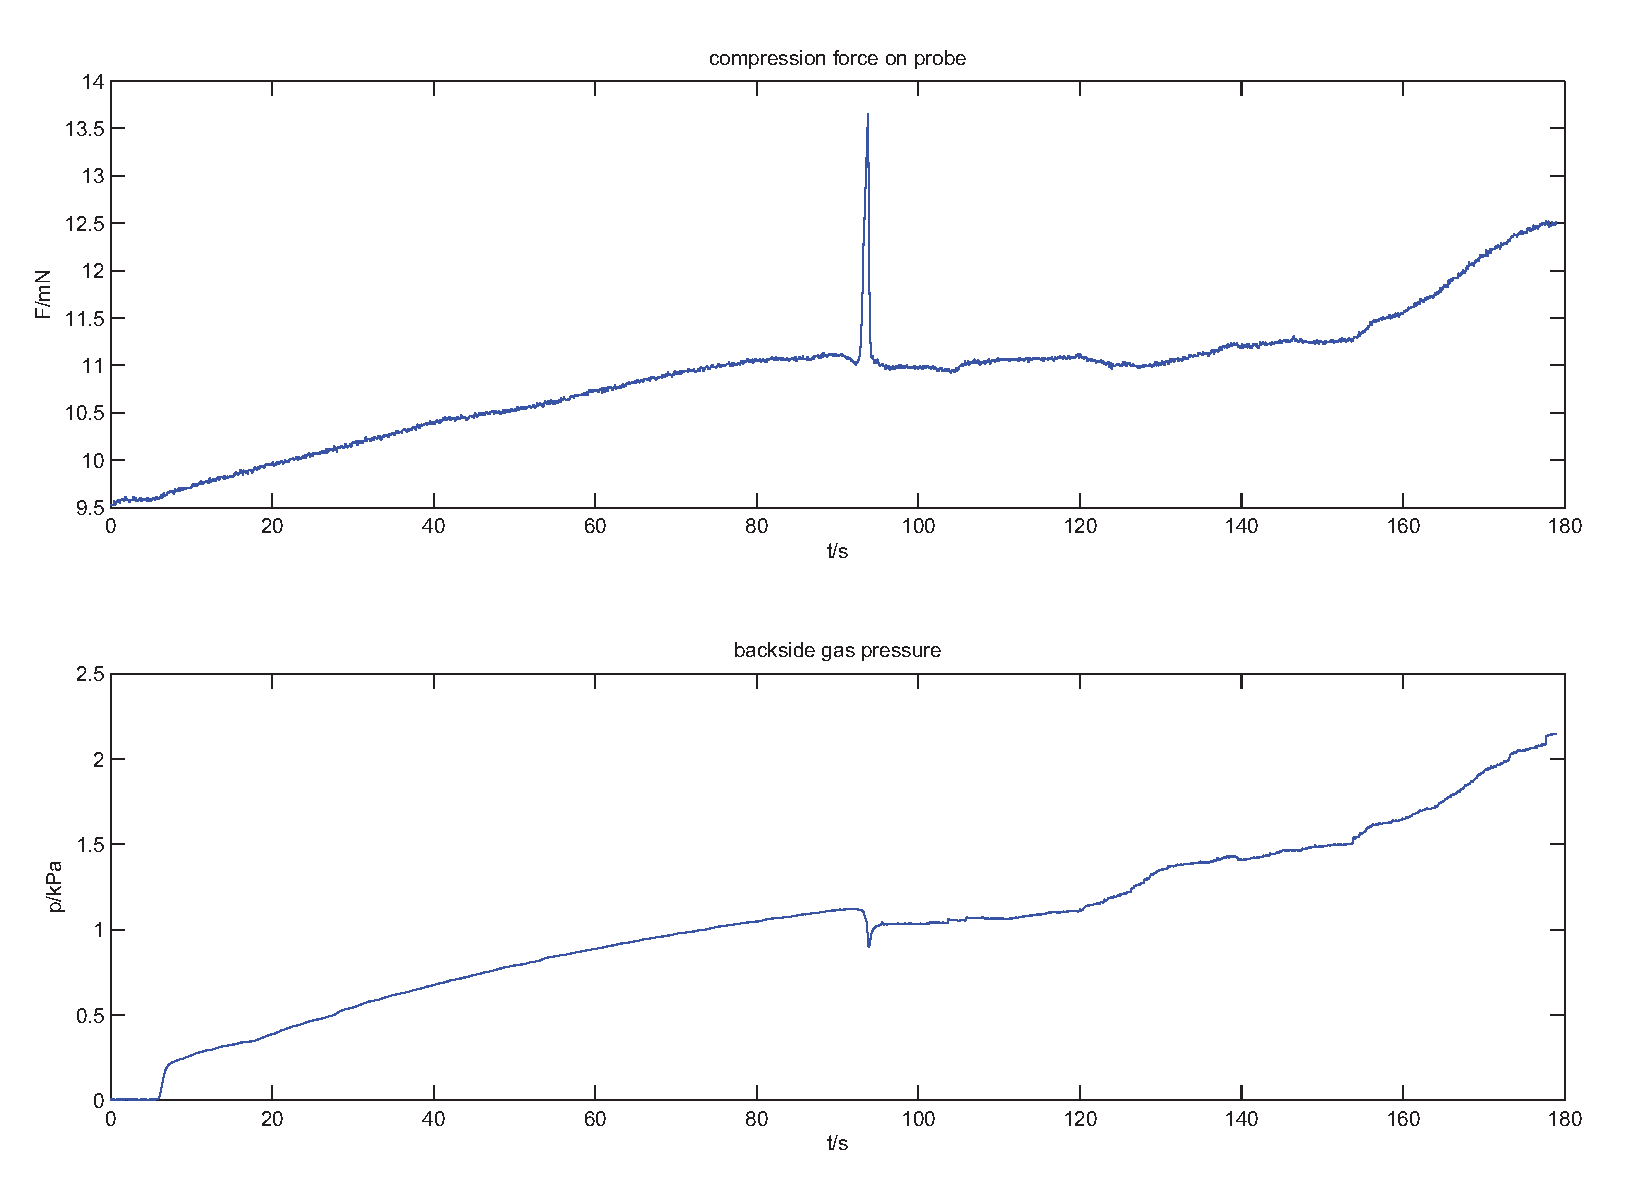
\includegraphics
  [max size={1\linewidth}{0.9\textheight}]
  {data/fpt__2400__2}
\caption{探头受力、背吹压强随时间变化曲线(样例1)}
\label{fig:data-fpt-2400-2}
\end{sidewaysfigure}

\begin{sidewaysfigure}[p]
\centering
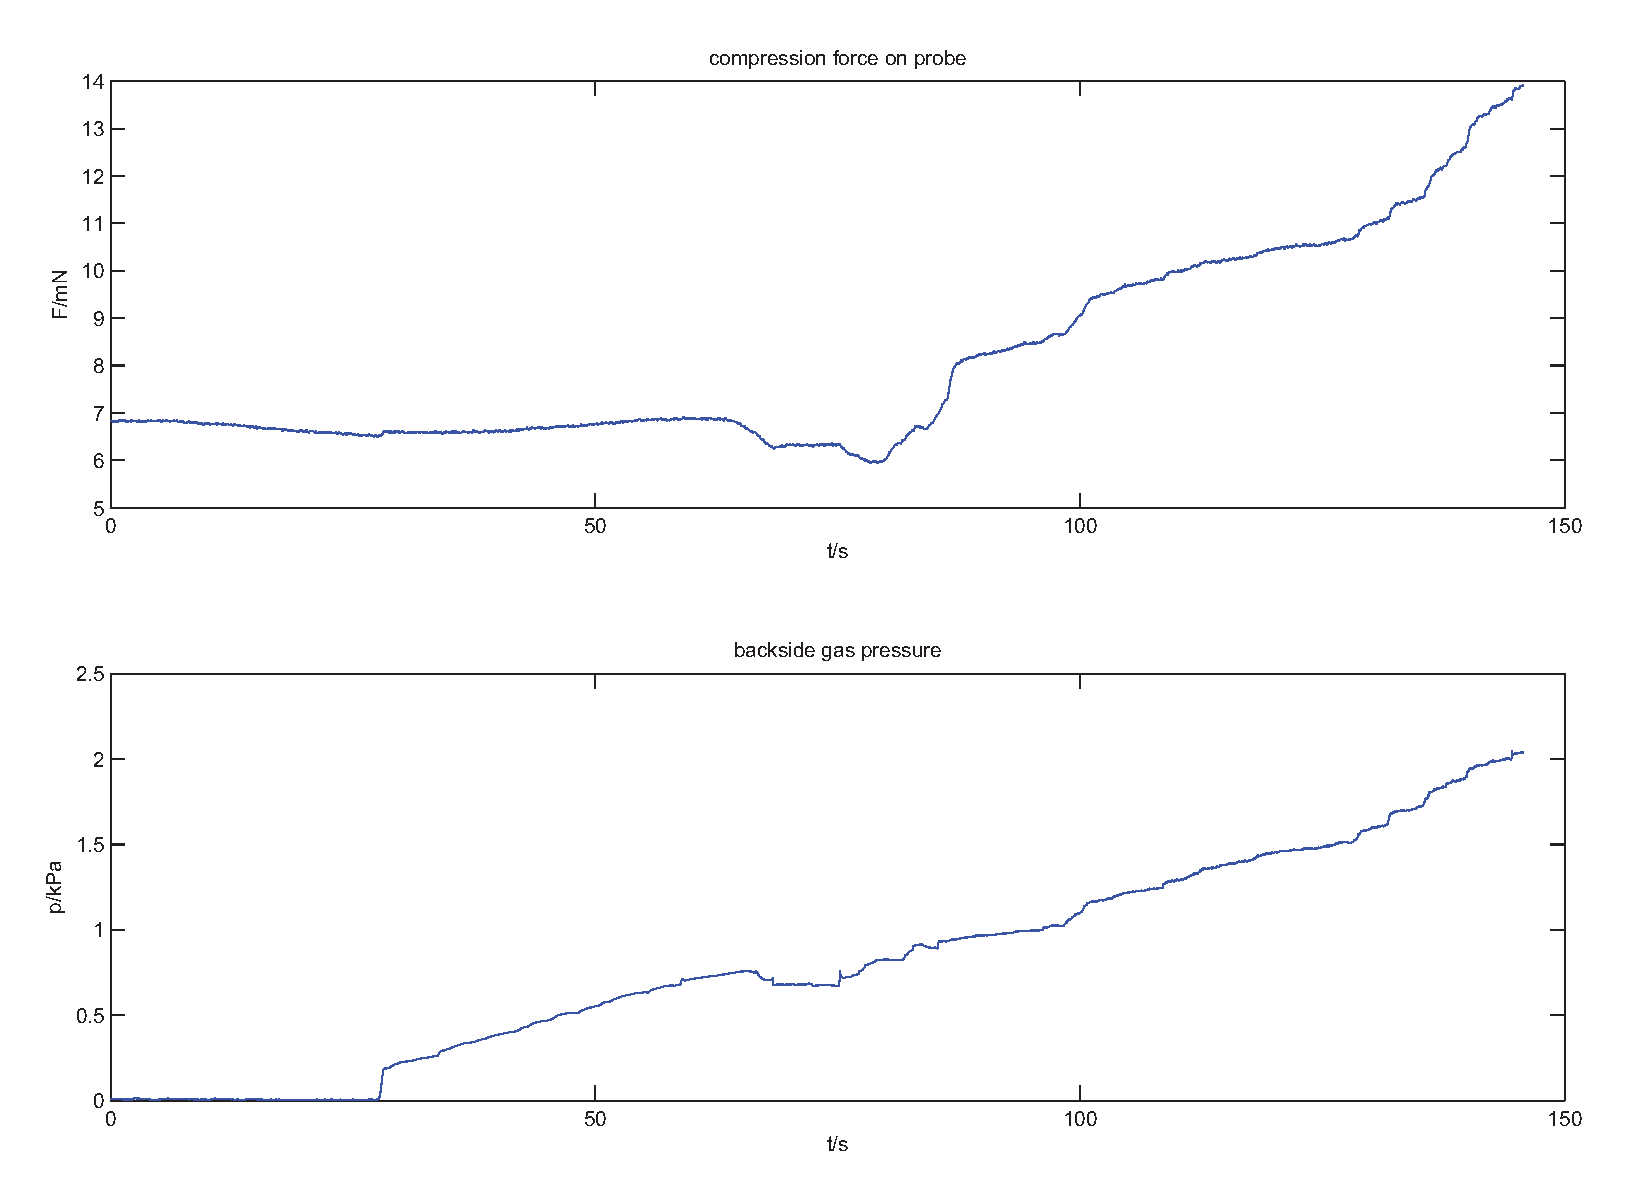
\includegraphics
  [max size={1\linewidth}{0.9\textheight}]
  {data/fpt__2200__5}
\caption{探头受力、背吹压强随时间变化曲线(样例2)}
\label{fig:data-fpt-2200-5}
\end{sidewaysfigure}

\begin{figure}[tbhp]
\centering
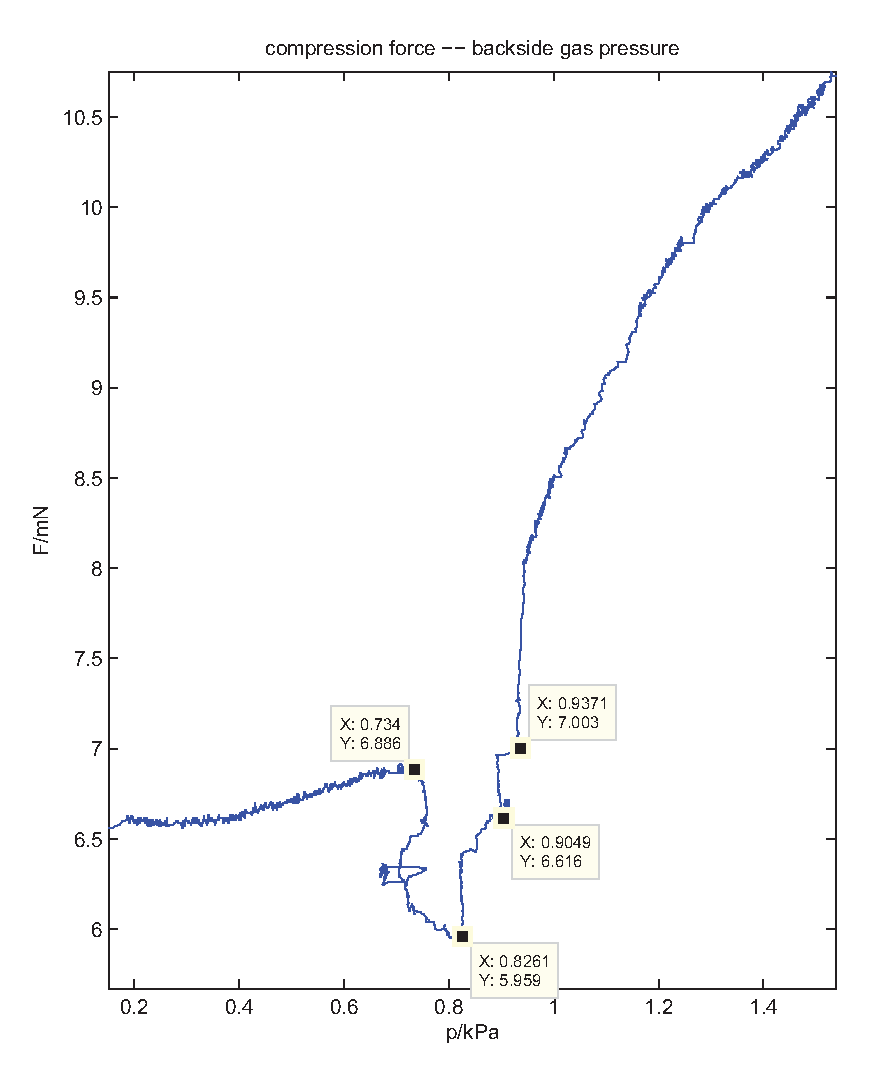
\includegraphics
  [max size={1\linewidth}{0.9\textheight}]
  {data/fp__2200__5}
\caption{探头受力随背吹压强变化曲线(样例2)}
\label{fig:data-fp-2200-5}
\end{figure}


\section{本章小结}\label{sec:exp-summary}




% !TeX root = ../main.tex
\cleardoublepage
\chapter{数据分析}\label{ch:analysis}

上一章的正式试验(\ref{sec:exp-main}节)中测得了\SIrange{1800}{2600}{\V}电压下的多组数据,并经初步处理得到$F$ -- $p$曲线以及关键点。本章将重点探讨这些数据所揭示出的晶圆脱附的物理过程,并据此判断出数据曲线中的晶圆脱附点,进而得到脱附背吹压强 -- 电压数据点。



\section{典型$F$ -- $p$曲线分析}\label{sec:analysis-example}


\subsection{简单型}\label{sec:analysis-example-naive} % 图样图森破,拿衣服

图~\ref{fig:data-fp-2000-4}、图\ref{fig:data-fp-2000-8}~所示的曲线明显可分为两部分:左下方的部分中,$p$缓慢上升的同时,$F$变化不大;而右方的部分中,$F$随$p$上升而快速上升;两部分中间有明显的转折点。除此转折点以外,可能还有其他的转折点,但对曲线整体走势影响不大。简单型曲线完全符合第\ref{ch:principle}章中对脱附判定的预测,然而实际情况表明,纯粹的简单型曲线占所有检测数据的比例非常小:虽然大部分数据走势与简单型类似,但其组成往往更复杂,在第一次出现$F$随$p$上升而快速上升(走势为向右上方)前后可能存在多个其他类型的转折点;这些特征将在其他曲线类型中介绍,并在\ref{sec:analysis-feature}节中加以分析。

\begin{figure}[tbh]
\centering
\includegraphics
  [max size={0.9\linewidth}{0.9\textheight}]
  {data/fp__2000__4}
\caption{探头受力随背吹压强变化曲线(\SI{2000}{\V} 第4组)}
\label{fig:data-fp-2000-4}
\end{figure}

\begin{figure}[p]
\centering
\includegraphics
  [max size={0.9\linewidth}{0.9\textheight}]
  {data/fp__2000__8}
\caption{探头受力随背吹压强变化曲线(\SI{2000}{\V} 第8组)}
\label{fig:data-fp-2000-8}
\end{figure}


\clearpage


\subsection{回转型}\label{sec:analysis-example-loop}

图~\ref{fig:data-fp-2400-2}、图\ref{fig:data-fp-2600-2}~所示曲线中能明显观察到一个大回环,其走向为逆时针方向,即:随着试验继续,$p$由逐渐升高转为降低\footnotemark{}的同时,$F$出现一个尖峰,又迅速回落。该特征在很多组数据曲线中均为最明显的特征之一,尤其是在电压较高($\geq \SI{2200}{\V}$)时。

\footnotetext{此时减压阀开度仍在增加,具体原因在后文中分析。}

\begin{figure}[tbh]
\centering
\includegraphics
  [max size={0.9\linewidth}{0.9\textheight}]
  {data/fp__2400__2}
\caption{探头受力随背吹压强变化曲线(\SI{2400}{\V} 第2组)}
\label{fig:data-fp-2400-2}
\end{figure}

\begin{figure}[p]
\centering
\includegraphics
  [max size={0.9\linewidth}{0.9\textheight}]
  {data/fp__2600__2}
\caption{探头受力随背吹压强变化曲线(\SI{2600}{\V} 第2组)}
\label{fig:data-fp-2600-2}
\end{figure}


\clearpage


\subsection{密集折点型}\label{sec:analysis-example-multi}

观察图~\ref{fig:data-fp-1800-10}、图\ref{fig:data-fp-2000-7}~所示曲线,发现虽然整体走势与\ref{sec:analysis-example-naive}节中简单型相似,但在两部分曲线中间出现多个相距不远的折点。其他数据曲线中,虽然较少出现与简单型相似的走势,仍有很多具有密集折点特征。

\begin{figure}[tbh]
\centering
\includegraphics
  [max size={0.9\linewidth}{0.9\textheight}]
  {data/fp__1800__10}
\caption{探头受力随背吹压强变化曲线(\SI{1800}{\V} 第10组)}
\label{fig:data-fp-1800-10}
\end{figure}

\begin{figure}[p]
\centering
\includegraphics
  [max size={0.9\linewidth}{0.9\textheight}]
  {data/fp__2000__7}
\caption{探头受力随背吹压强变化曲线(\SI{2000}{\V} 第7组)}
\label{fig:data-fp-2000-7}
\end{figure}


\clearpage


\subsection{倒勾型}\label{sec:analysis-example-sawtooth}

图~\ref{fig:data-fp-2400-6}、图\ref{fig:data-fp-2600-5}~所示的曲线走势与大部分数据曲线不同:在检测刚开始的时候,$F$即随$p$上升而上升,然后在一点突然出现转折,曲线总体趋势变为$p$上升而$F$反而快速下降。

\begin{figure}[tbh]
\centering
\includegraphics
  [max size={0.9\linewidth}{0.9\textheight}]
  {data/fp__2400__6}
\caption{探头受力随背吹压强变化曲线(\SI{2400}{\V} 第6组)}
\label{fig:data-fp-2400-6}
\end{figure}

\begin{figure}[p]
\centering
\includegraphics
  [max size={0.9\linewidth}{0.9\textheight}]
  {data/fp__2600__5}
\caption{探头受力随背吹压强变化曲线(\SI{2600}{\V} 第5组)}
\label{fig:data-fp-2600-5}
\end{figure}


\clearpage


\subsection{复合型}\label{sec:analysis-example-complex}

正式试验获得的数据中,还有一些曲线中同时呈现出多个特征,如:图~\ref{fig:data-fp-2200-6}、图~\ref{fig:data-fp-2200-7}~均可视为倒钩型、回转型、简单型的顺序组合;图~\ref{fig:data-fp-2400-7}可视为倒钩型、密集折点型与简单型的顺序组合等等。这类数据揭示了背吹平衡脱附过程本身的复杂性,需通过对其组成特征的分析来加深对其内在物理过程的理解。

\begin{figure}[tbh]
\centering
\includegraphics
  [max size={0.9\linewidth}{0.9\textheight}]
  {data/fp__2200__6}
\caption{探头受力随背吹压强变化曲线(\SI{2200}{\V} 第6组)}
\label{fig:data-fp-2200-6}
\end{figure}

\begin{figure}[tbh]
\centering
\includegraphics
  [max size={0.9\linewidth}{0.9\textheight}]
  {data/fp__2200__7}
\caption{探头受力随背吹压强变化曲线(\SI{2200}{\V} 第7组)}
\label{fig:data-fp-2200-7}
\end{figure}

\begin{figure}[p]
\centering
\includegraphics
  [max size={0.9\linewidth}{0.9\textheight}]
  {data/fp__2400__7}
\caption{探头受力随背吹压强变化曲线(\SI{2400}{\V} 第7组)}
\label{fig:data-fp-2400-7}
\end{figure}



\clearpage



\section{曲线特征与对应物理过程}\label{sec:analysis-feature}




\subsection{失稳性脱附}\label{sec:analysis-feature-destabilize}

当类似\ref{sec:analysis-example-naive}节中图~\ref{fig:data-fp-2000-4}~所示的$p$较小增长引起$F$较大增长的曲线段出现时,可认为是微力探头与晶圆接触处局部已发生决定性的脱附,即随着静电力减小,间隙随之逐渐扩大,引起静电力进一步减小,仅由于晶圆本身刚度以及其他区域吸附力的影响,尚未完全脱附,此时再增加压强,则未能与静电力相平衡的压力将由微力探头对晶圆施加的接触力来平衡。

%TODO:more features



\section{脱附点的判定}\label{sec:analysis-criterion}

%TODO:criterion




\section{数据汇总与拟合}\label{sec:analysis-tally}

按照上文总结出的数据处理与分析方法,求出正式试验中所有有效数据的脱附压强,并对同电压下的多组数据取中位数\footnotemark{}后,用二次多项式拟合,结果如图~\ref{fig:data-tally},多项式为:
\[
\hat{p} = 0.05919\;\hat{v}^2 + -1.324\;\hat{v} + 1.000
\]
其中,$\hat{p} = p / \SI{1}{\kPa}$,$\hat{v} = v / \SI{1}{\kV}$。拟合相关系数$R^2 = \num{0.9992}$
虽然相关系数较高,说明数据较好地符合拟合多项式,但考虑到在库仑型静电卡盘的静电力理论公式中
%TODO:xref bg eqn
,静电力与电压平方成正比,无法解释拟合多项式中的一次项,说明实际静电力产生机理比理论公式复杂,仍有理论公式未能考虑到的因素。

\footnotetext{由于数据点较分散,用中位数能更准确地估计某一电压下的脱附压强真实值。}

\begin{figure}[thbp]
\centering
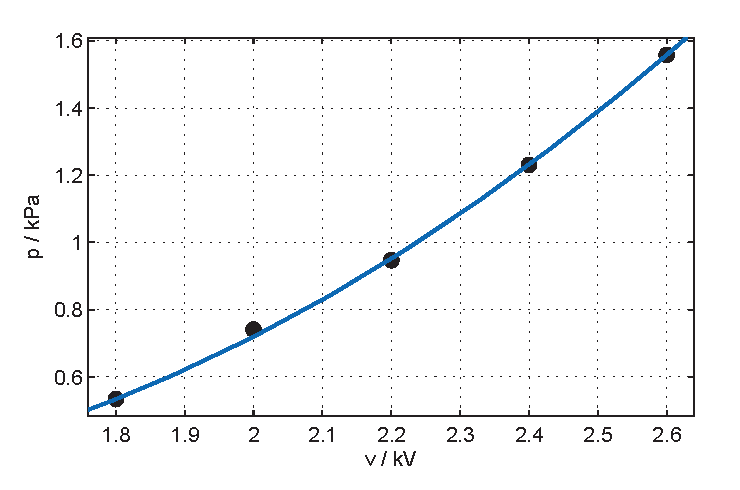
\includegraphics[width=0.8\linewidth]{data/tally}
\caption{脱附背吹压强 -- 电极电压数据点汇总与拟合}
\label{fig:data-tally}
\end{figure}



\section{本章小结}\label{sec:analysis-summary}



%% !TeX root = ../main.tex
\cleardoublepage
\chapter{结论}\label{ch:conclusion}


\section{论文的主要成果与创新点 }\label{sec:conclusion-review}

本文通过分析现有静电卡盘静电力检测方案中存在的检测准确性与可重复性等问题,自主提出了一种改进方案,设计并搭建了一套完整的静电卡盘静电力检测软硬件平台,提出了一种利用该平台自动化检测静电力的方法及其规范流程。通过分析气体背吹压力与微力探头受力的相关性,深入探讨了晶圆多种脱附过程的作用机理以及脱附时刻的判断方法。本研究的主要成果与创新点如下:

\begin{enumerate}
  \item 针对背吹平衡法中气隙扩大、晶圆变形等影响静电力检测准确性的诸多不利因素,提出一种利用微力探头检测、控制并消除气隙变化的方法,可准确地判断脱附时刻,并在一定程度上揭示了晶圆脱附过程的复杂性。同时提出了一种利用重力平衡原理标定背吹压强等效作用面积的方法,为进一步探究静电卡盘中复合场耦合作用提供支持。
  \item
  已有研究对晶圆脱附过程作出诸多假设,如静电力随间隙增加而降低、背吹气层在晶圆下表面压强均匀分布等,而本文实验研究表明晶圆实际脱附过程远比假设复杂的多,本文对实际测得的脱附过程进行了归纳与解释,并深入探讨了判断脱附时刻的一般性方法。
  \item 为提高检测准确性和检测效率,本文设计并实现了静电卡盘静电力检测流程的电控与自动化,可在较短时间内获得大量有效数据,为深入研究静电力产生与消除机理提供了必要的软硬件基础。
\end{enumerate}



\section{工作展望}\label{sec:conclusion-future}

由于时间、条件所限,本研究中提出的检测方案仍有改进余地。首先,如\ref{sec:exp-main-proc}节所述,试验条件若能全部实现,预计试验的可重复性与准确度均会有较大提升。检测方案中的重力平衡法未能实际实现,其主要原因是因为发现“压强作用等效面积”在复杂的脱附过程中可能并非常量,而可能与具体的脱附过程有关,导致标定该量的方法需要做进一步研究。

检测平台的设计与实现也有较大的改进空间:检测平台中的背吹控制系统仍不完善,现在完全依靠机械式减压阀来供压,应在未来的工作中,选用更合适的电子比例阀或压力控制器,甚至实现反馈控制泵式压力控制器等,以实现背吹供压的自动化。另外,由于本研究带有探索性质,电控系统未能实现更高的集成度,目前仍是较多模块松散连接的方式,可以考虑在检测平台定性之后,按照本文中的原理方案,改进电控系统的具体设计与实现。

由于脱附过程极为复杂,仅靠一个微力探头得出的数据难以反映整个晶圆面积上发生的物理过程全貌,考虑在后续试验中,在圆周对称的位置上加装微力探头,或增加激光测距仪/干涉仪等,获得更多关于晶圆在脱附过程中局部受力与形变的数据,以此加深对脱附过程的理解。

现有的商业有限元仿真软件(ANSYS、COMSOL等)均无法较好地建立同时考虑机械接触与背吹气体流动的静电卡盘力学模型,因此本工作未能包括试验数据与仿真结果的对比研究。若能开发出准确建模该系统的仿真方法,则可更好地揭示脱附过程中整个系统内部发生的不易观察、检测的物理过程,获得对晶圆脱附、吸附、乃至整个静电卡盘设计优化的更清楚的认识。



%%% 其它部分
\backmatter

% 本科生要这几个索引,研究生不要。选择性留下。
\makeatletter
\ifthu@bachelor
  % 插图索引
  \listoffigures
  % 表格索引
  \listoftables
  % 公式索引
  %\listofequations
\fi
\makeatother


% 参考文献
\bibliographystyle{thubib}
\bibliography{ref/refs}


% 致谢
\begin{ack}
感谢我的指导老师,同时也是我的班主任程嘉老师。从上学期开题以来,程老师一直支持、鼓励我探索具有新颖性、创新性的检测方案,每周耐心地与我讨论项目进展,并引导我与实验室的老师同学和华卓精科公司的工程师交流思想,虚心听取意见建议;整个研究的工作量庞大,在程老师的合理规划下,每一部分的工作才得以有条不紊地按时完成。

在检测平台的设计阶段,我在制造所的吴丹老师的启发下,确定了微力探头的总体设计思路;在制造所的杨开明老师的指导下,在大量产品中选择出了最适合检测平台要求的电动推杆。在此感谢两位老师对我的热情帮助。

加入课题组以来,王珂晟、王兴阔师兄与曹明路师姐一直热情地支持着我的工作,给予了我很多帮助;他们之前做过的工作也为我的检测方案以及试验过程的具体设计提供了很多启发。两位师兄更是抽出了大量时间帮助我完成了最关键的两次试验。

我的研究中使用的静电卡盘从华卓精科公司获得,由北方微电子公司提供。所有机加工件均由华卓精科公司代送外协加工。在此感谢华卓精科许岩经理与张旭光工程师在检测方案设计、检测平台的搭建与调试等阶段给予我的支持与鼓励。还要感谢北方微电子公司的栾大为工程师提供有关待测静电卡盘的准确而详细的技术资料。

在电控系统的具体设计与实现上,清华大学学生创新社(AOI)的张骏琳同学、吴天际学长、以及幻腾智能团队的郎朝见工程师提出了许多宝贵的参考意见,帮助我在较短的时间内解决了电控系统从设计到实现中的各种问题。在此感谢他们无私的帮助。

感谢WIKA中国的汪博工程师在背吹控制系统方面无私提供的宝贵的意见,虽然最后未能使用WIKA产品,这些意见对背吹控制系统最终能够达到检测平台要求起到了至关重要的作用。
\end{ack}


% 附录
\begin{appendix}
% !TeX root = ../main.tex
\cleardoublepage

%%% translation-related manual formatting
\newcommand{\apptitle}[1]{\parbox{0.9\linewidth}{\centering #1}\par\bigskip}
\newcommand{\appfigref}[2]{图~#1 -- #2~}
\newcommand{\appcite}[1]{\par\bigskip\apptitle{原文索引}\noindent\parbox{1\linewidth}{\small #1}}
\chapter{外文资料的书面翻译}

\apptitle{感性耦合等离子体环境下的静电卡盘特性瞬态分析}

\noindent 摘要:本文分析了感性耦合等离子体(ICP)环境下,用于在半导体工艺过程中夹持硅晶圆的J-R型静电卡盘(ESC)。我们提出了一个静电卡盘的双层等效电路模型,其组成为一较厚的整体层和一较薄的界面层。通过测量有/无晶圆时静电卡盘的伏安特性,可算出各层的等效电阻值,以及界面层两端等效电压。在静电卡盘上施加一斜坡电压信号,并测量其瞬态电流,积分即可得到界面层等效电容中储存的电荷量。另外,我们通过缓慢降低电压而使晶圆在氦气背吹作用下脱离卡盘的方式,在原位测量出了静电卡盘施加的静电力。用我们提出的等效电路模型预测的静电力与实际测量出的静电力相吻合。

\par\bigskip

\noindent \textbf{关键词:}J-R型;静电卡盘;感性耦合等离子体;双层模型

\par\bigskip

在有等离子体参与的半导体制程中,静电卡盘广泛用于真空环境中夹持硅晶圆。常用的静电卡盘分两种:库仑型[1-3],特点是使用绝缘体电介质层(体积电阻率$\rho > \SI{1e14}{\ohm\cm}$);以及Johnsen-Rahbek(J-R)型,特点是使用半导体电介质层($\rho = \SIrange{1e10}{1e12}{\ohm\cm}$)。静电吸附力由晶圆与静电卡盘中电极在高压作用下产生的异号电荷相吸引产生。与库仑型相比,J-R型静电卡盘可在较低电压下产生较强的吸引力,其原因主要是介电层表面微观不平度与晶圆接触后,缝隙间产生强电场。但J-R型静电卡盘吸附机理较复杂,且对界面层中的很多物理参数敏感,如电导率,表面微观不平度(亚显微级),甚至电极/晶圆的宏观平面度等;并且,使用J-R型静电卡盘的工艺存在一系列问题,如残余电荷带来的较差的可重复性,静态电流造成的晶圆表面镀膜破坏,以及将晶圆从静电卡盘表面卸下时,由顶针和残余电荷作用产生的晶片破损等。

为了能够消除这些缺点,我们需要增进对J-R型静电卡盘的理解,尤其是在等离子存在的实际工况下。在之前发表的文献[6]中,我们提出了射频偏压对低密度容性耦合等离子体(CCP)条件下的静电卡盘的伏安特性的影响。这里我们提出在高密度感性耦合等离子体(ICP)条件下的瞬态分析。接通电压时的瞬态电流的积分即为界面层电荷量,缓慢关断电压时,通过检测氦气背吹流量变化可测出静电吸附力。我们提出的双层等效电路模型可解释J-R型静电卡盘的特性。

实验使用一套ICP反应腔室[7],其圆柱形不锈钢制腔室中,使用\SI{13.56}{\MHz}射频放电激发\SI{0.1}{\torr}压强下的\ce{Ar}产生等离子体。在腔室内装有一\SI{200}{\mm}直径的J-R型静电卡盘。静电卡盘的电极材料为\ce{Mo},镶嵌在\SI{5}{\mm}厚的\ce{AlN}电介质层中,与接触表面距离\SI{0.54}{\mm}。接触表面总面积为电极投影面积的60\%(直接与晶圆接触的是静电卡盘表面上的凸台,高\SI{50}{\um},长宽\SI{2}{\mm},主要作用是为氦气冷却提供通道)。

\begin{figure}[tbhp]
\centering
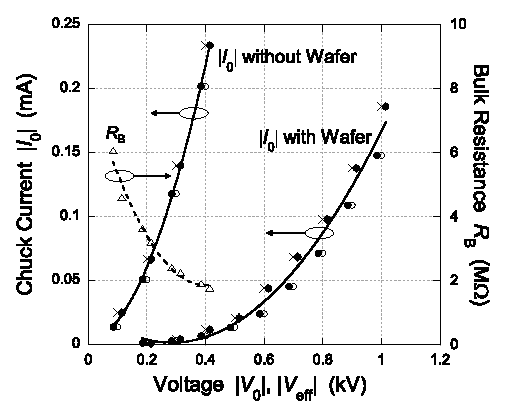
\includegraphics[width=0.7\linewidth]{_a/nagoya__1}
\caption*{图~A -- 1\hspace{1em}在有/无晶圆时,$I_0$与$\left|V_0\right|$的关系,以及无晶圆时$R_{\mathrm{B}}$的大小}
\end{figure}

首先,我们测量了\SI{600}{\W}放电,\SI{0.1}{\torr}压强产生的\ce{Ar}等离子体条件下,通过静电卡盘流向一直径\SI{200}{\mm}的硅晶圆的电流$I_0$与静电卡盘电压$V_0$(\SI{-1}{\kV}到\SI{+1}{\kV}之间)的函数关系。如\appfigref{A}{1}中``$\circ$''与``$\times$''所示,电压绝对值相同时,电流绝对值$\left|I_0\right|$在电压为负值时比电压为正值时要大。这个现象可用自偏压现象(self-bias effect)解释[6]:晶圆表面在ICP作用下,具有表面电势$V_{\mathrm{W}} \sim \SI{12}{\V}$,因此实际上静电卡盘中电极与晶圆之间的有效电压为$V_{\mathrm{eff}} = V_0 - V_{\mathrm{W}}$;即,$\left|V_0\right|$相等时,$-\left|V_0\right|$对应的有效电压更大。\appfigref{A}{1}中``$\cdot$''即为将电压修正为$V_{\mathrm{eff}}$的结果。$V_{\mathrm{eff}}/I_0$即为总电阻$R_{\mathrm{T}}$,由\ce{AlB}整体区电阻$R_{\mathrm{B}}$和接触电阻组成。%
当$\left|V_0\right|=\SI{0.4}{\kV}$时,$R_{\mathrm{T}} \sim \SI{40}{\Mohm}$;%
当$\left|V_0\right|=\SI{0.7}{\kV}$时,$R_{\mathrm{T}} \sim \SI{10}{\Mohm}$;%
当$\left|V_0\right|=\SI{1.0}{\kV}$时,$R_{\mathrm{T}} \sim \SI{6}{\Mohm}$;%
但这些数值明显大于通过体积电阻率估计出的整体层电阻$R_{\mathrm{B}} \sim \SI{3}{\Mohm}$(设$\rho=\SI{2e10}{\ohm\cm}$)。

通过测量观察到的在低电压下的高总电阻值说明在晶圆与静电卡盘中间存在较大的接触电阻。为了测出该接触电阻,首先要测量整体层电阻。将静电卡盘表面直接暴露在等离子体下,不加晶圆,测得其伏安特性如\appfigref{A}{1}。由于等离子体与静电卡盘接触较好,低电压下测得的电流较高。此时,整体层电阻即为$R_{\mathrm{B}}=\left|V_{\mathrm{eff}}\right| / \left|I_0\right|$,在\appfigref{A}{1}中用``$\Delta$''表示,可达\SI{2}{\Mohm}($V_0 > \SI{0.2}{\kV}$)。随着电压降低,仍可观测到电阻升高,这可能是由于静电卡盘与等离子体中仍存在的接触电阻升高造成的。

\begin{figure}[tbhp]
\centering
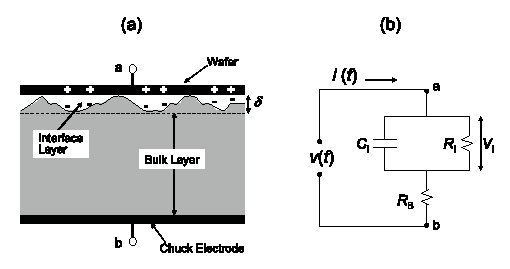
\includegraphics[width=0.7\linewidth]{_a/nagoya__2}
\caption*{图~A -- 2\hspace{1em}(a)\ J-R型静电卡盘双层模型\quad (b)\ 其等效电路}
\end{figure}

由\appfigref{A}{1}所示的测量数据,总结出\appfigref{A}{2}所示的J-R型静电卡盘双层模型,及其等效电路模型(\appfigref{A}{2(b)})。可将电极与晶圆之间的\ce{AlN}分为厚度$l=\SI{0.54}{\mm}$的整体层,其电阻为$R_{\mathrm{B}}$;以及厚度为$\delta$,较薄的界面层,其电阻为$R_{\mathrm{I}}$,电容为$C_{\mathrm{I}}=\varepsilon_0 S_{\mathrm{I}} / \delta$($S_{\mathrm{I}}$为待定的电容等效面积)。由于$\delta \ll l$,整体层的电容可忽略。总电阻$R_{\mathrm{T}}=R_{\mathrm{B}}+R_{\mathrm{I}}$。由伏安特性可知,$R_{\mathrm{I}}$随有效电压$V_{\mathrm{eff}}$非线性变化;这是J-R效应影响造成的,其机理可归结为在强电场下的电子场致发射现象[7,9,10]。整体层中流过的电流分布较均匀,但在通过界面层的若干个不规则接触点时,产生不均匀分布,并在接触点附近留下表面电荷$Q_0$;这样,晶圆与静电卡盘上的异号电荷形成了真空中的分布电容,其平均间隙为$\delta$;静电吸附力由此产生。随时间丢失的电荷由静态电流$I_0$补充,因此有如下稳态方程:
\begin{equation}\tag*{(A-1)}\label{eq:-a-1}
V_{\mathrm{I}}=R_{\mathrm{I}} I_0
Q_0=C_{\mathrm{I}} V_{\mathrm{I}}
\end{equation}

\begin{figure}[tbhp]
\centering
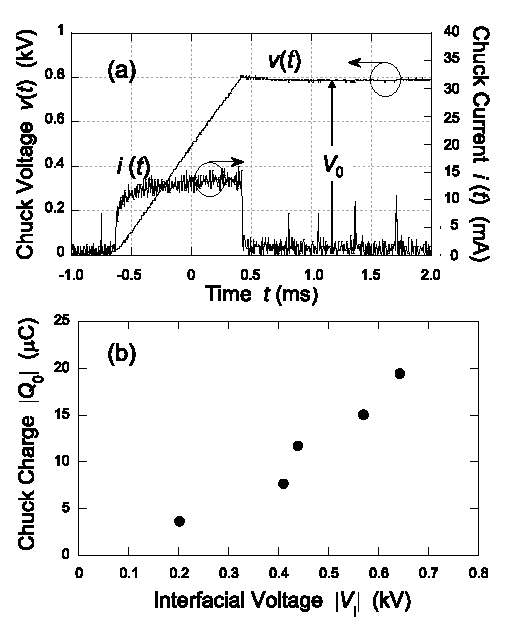
\includegraphics[width=0.5\linewidth]{_a/nagoya__3}
\caption*{图~A -- 3\hspace{1em}(a)\ $v(t)$与$i(t)$随时间变化\quad (b)\ 卡盘电荷$\left|Q_0\right|$随界面层电压$V_{\mathrm{I}}$变化关系 (\SI{600}{\W}、\SI{0.1}{\torr}条件下)}
\end{figure}

\begin{figure}[tbhp]
\centering
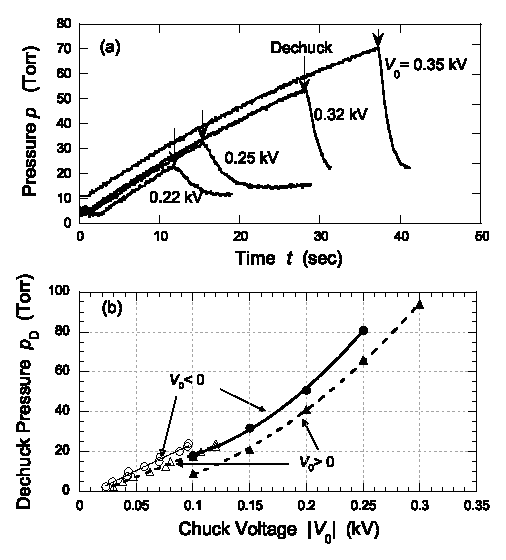
\includegraphics[width=0.5\linewidth]{_a/nagoya__4}
\caption*{图~A -- 4\hspace{1em}(a)\ 流量为\SI{10}{\sccm},电压不同时的氦气压强随时间变化关系\quad (b)\ 脱附压强随电压关系,负$V_0$为圆形点,正$V_0$为三角形点,恒流量法为实心点,恒压强法为空心点}
\end{figure}

为了得到稳态电荷$Q_0$,可在静电卡盘上施加一斜坡电压信号,并测量流过静电卡盘的瞬态电流,如\appfigref{A}{3(a)},电压$V_0$在$\tau_{\mathrm{R}} \sim \SI{1}{\ms}$内从0线性上升到\SI{0.8}{\kV}。电压关断时测得结果与接通时基本相同,只是电流方向相反(未在图中画出)。在图中,$\SI{-0.4}{\ms}<t<\SI{+0.4}{\ms}$时,可观测到较大(\SI{13}{\mA})的充电电流,之后迅速降到很小的稳态电流值(\SI{0.08}{\mA});偶尔出现的电流尖峰可能是由限流元件产生的。将测得的瞬态充电电流积分即可得到静电卡盘表面电荷量$Q_0$。如此可测得各电压$V_0$($<0$)下的表面电荷数据。定义界面层电压$V_{\mathrm{I}} = V_{\mathrm{eff}} - R_{\mathrm{B}} I_0$(即等效电路图中$C_{\mathrm{I}}$与$R_{\mathrm{I}}$两端的电压),其与$Q_0$关系如\appfigref{A}{3(b)}。可见,电荷量与电压并不成正比,其等效电容$C_{\mathrm{I}} = \left|Q_0\right| / \left|V_{\mathrm{I}}\right|$,在电容两端电压%
为\SI{0.2}{\kV}时为\SI{18}{\nano\farad},%
在\SI{0.64}{\kV}时为\SI{30}{\nano\farad}。%
这种电容随电压上升的现象,我们暂时认为是由于电压升高导致静电力升高,使得界面层厚度$\delta$缩小造成的。

通过原子力显微镜测量得到硅晶圆的表面粗糙度为\SIrange{0.8}{1.6}{\um}。考虑到介电层表面与晶圆表面的微观与宏观不平度,我们估计在电压为\SI{0.2}{\kV}时,界面层平均厚度$\delta \sim \SI{5}{\um}$;此时$C_{\mathrm{I}}=\SI{18}{\nano\farad}$,得到电容等效面积$S_{\mathrm{I}} \sim \SI{1.02e-2}{\m^2}$。另外,由于表面凸台影响,介电层与晶圆的实际接触面积为\SI{200}{\mm}直径圆形晶圆的60\%\footnotemark{},即$S_*=\SI{1.88e-2}{\m^2}$。

\footnotetext{译者注:此处原文意为“减小60\%接触面积”,有误,根据前后数据推断,实际应为“接触面积为整个晶圆的60\%”。}

为了检测静电吸引力,我们将一定压强的氦气通入晶圆与静电卡盘之间的空隙中。当作用在晶圆上的气体向上的压力稍微超过静电吸附力时,晶圆将脱离静电卡盘表面;此时氦气压力和/或流量将会发生改变。我们采用了两种测量方式:恒流量法和恒压强法。

如\appfigref{A}{4(a)},恒流量法是将氦气以固定的质量流量(\SI{10}{\sccm},即标况下\SI{10}{\cm^3\per\s})通入静电卡盘;共测试了4组电压下的情况:\SIlist[list-separator={,},list-final-separator={,以及}]{0.22;0.25;0.32;0.35}{\kV}。随着氦气流入,其压强逐渐升高;晶圆脱离后,由于气体大量漏出,压强突然降低。因此,图中标出的压强最高值,即晶圆即将脱离时的压强$p_{\mathrm{D}}$,就是气压与静电力平衡时的压强。\appfigref{A}{4(b)}中``$\bullet$''与``$\Delta$''分别表示$V_0 < 0$与$V_0 > 0$时,$p_{\mathrm{D}}$与$\left|V_0\right|$的关系。可见$V_0 < 0$时,吸附力更大。图中实线与虚线分别是两组数据的拟合曲线;其距离大约是\SI{25}{\V},与$V_{\mathrm{W}}$二倍大致相当,符合之前由\appfigref{A}{1}得出的结论。

在一系列试验过程中,我们发现前一次实验的结果会严重影响后一次,其原因为:当晶圆脱离后,在静电卡盘表面仍残留部分表面电荷,而这些电荷会影响后续试验。为了保证试验可重复性,我们在晶圆脱离后,将脱离的晶圆移至真空交换室(load-lock chamber),然后将静电卡盘暴露在\SI{0.1}{\torr}压强的\ce{Ar}等离子体中\SI{30}{\s},以去掉其表面残余电荷;这样即可保证采集数据可靠性。

\begin{figure}[tbhp]
\centering
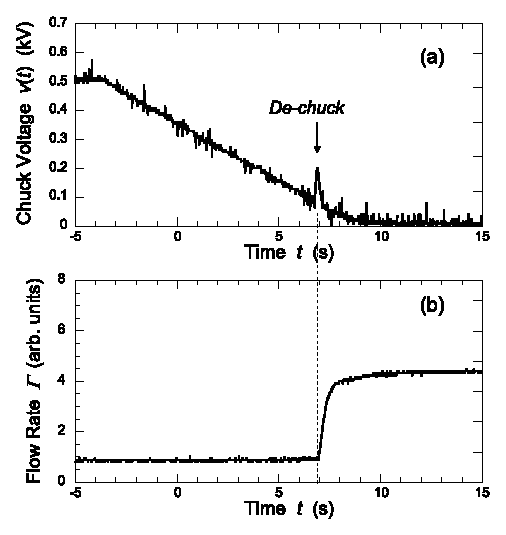
\includegraphics[width=0.7\linewidth]{_a/nagoya__5}
\caption*{图~A -- 5\hspace{1em}(a)\ $v(t)$随时间变化\quad (b)\ 氦气流量$\Gamma$随时间变化}
\end{figure}

在电压较低($\left|V_0\right| < \SI{0.15}{\kV}$)时,由于信号较小,而扰动较大,恒流量法测试精度下降。因此,在低电压区我们改用恒压强法来检测静电力。如\appfigref{A}{5},在维持氦气压力一定时,缓慢降低静电卡盘电压。氦气压强维持在$p = \SI{10}{\torr}$时,电压$V_0$在$t=\SI{-3.5}{\s}$时开始由\SI{0.5}{\kV}缓慢下降(约需10 s降至\SI{0}{\V})。\appfigref{A}{5(b)}中可见,在$t=\SI{7}{\s}$时,氦气流量突然增加,说明此时晶圆脱离,对应电压为\SI{0.07}{\kV}。脱离后,氦气流量迅速达到流量控制器允许的最大流量(\SI{50}{\sccm})。另外,在脱离时,可观测到电压值也出现一个尖峰,这是阻抗发生变化造成的。

当设置氦气恒定压强高于\SI{10}{\torr}时,晶片更早脱离,说明脱离时静电卡盘电压更大。反复试验即可得到气压与电压的函数关系,如\appfigref{A}{4(b)}中``$\circ$''和``$\Delta$''所示。当$\left|V_0\right|=\SI{0.1}{\kV}$时,更准确的恒定压强法获得的$p_{\mathrm{D}} \sim \SI{20}{\torr}$,约是恒流量法测试结果的两倍。

气体压强作用在晶圆上的面积$S_{\mathrm{M}}=\SI{1.26e-2}{\m^2}$(\SI{200}{\mm}直径晶圆的40\%)\textit{,除了电容等效面积$S_{\mathrm{I}}$}\footnotemark{}。因此,气压作用在晶圆上的合力为
\begin{equation}\tag*{(A-2)}\label{eq:-a-2}
F_{\mathrm{M}} = p_{\mathrm{D}} S_{\mathrm{M}}
\end{equation}
另一方面,使用测量得到的电容模型,可估计静电力为:
\begin{equation}\tag*{(A-3)}\label{eq:-a-3}
F_{\mathrm{E}} = \frac{D^2}{2 \varepsilon_0} S_{\mathrm{I}}
\end{equation}
其中电位移$D=Q_0/S_{\mathrm{I}}$。当静电卡盘电压$\left|V_0\right|=\SI{0.1}{\kV}$时,较准确的恒压强法测得$p_{\mathrm{D}} \sim \SI{20}{\torr}$,可得$F_{\mathrm{M}} \sim \SI{33.5}{\N}$;同条件下测得的表面电荷量$Q_0 \sim \SI{2.5}{\micro\coulomb}$,可得$F_{\mathrm{E}} \sim \SI{35.3}{\N}$。两者相差不大,在实验误差允许范围内,验证了晶圆脱离时$F_{\mathrm{M}}=F_{\mathrm{E}}$这一关系。

\footnotetext{译者注:原文此处语法不通,且由后面计算推断,此处并未从$S_{\mathrm{M}}$中扣除$S_{\mathrm{I}}$。}

总结:我们分析了ICP反应腔室中J-R型静电卡盘的基本特性,提出了由较厚阻性层与较薄容性层构成的双层电路模型,并通过加/不加晶圆的方法,用伏安特性法测量出了每一层的电阻值。加电压时的瞬态测量提供了一种新的测量静电卡盘表面电荷量的方式,并间接提供了估计静电力的方式(静电力与电荷量平方成正比)。我们还提出了一种利用氦气加压的较为精确地在原位测量静电力的方式;该法测量出的静电力与等效电路模型估测出的静电力相符较好。

\appcite{[1] SHIM G. I., SUGAI H. Temporal Analysis of Electrostatic Chuck Characteristics in Inductively Coupled Plasma[J]. Plasma and Fusion Research, 2008, 3: 028-028.} 


\clearpage


\apptitle{对夹持硅晶圆用的静电卡盘的基础研究}

\noindent 摘要:在半导体工业中,机械夹持晶圆的装置可能导致严重的问题。改用静电卡盘是可能解决这些问题的一种途径。我们研究了由交错电极和薄膜介电层组成的静电卡盘对硅片产生的静电吸引力的规律。当电压上升或介电层厚度降低时,静电力均上升。当交错电极的宽度和间距降低时,也能获得更强的静电力。实验表明当电极宽度和间距均为\SI{1}{\mm}、介电层为\SI{50}{\um}时,可获得最强的静电力:电压3.7 kV、吸引4英寸晶圆时,竖直方向静电力约为\SI{17}{\N}。在施加高压直流电压后,即使撤去电压,仍存在一些残余静电力,这种效应可用施加变频交流高压电的方式解决。

\par\bigskip

\noindent \textbf{关键词:}薄膜介电层;静电卡盘;静电力;硅晶圆夹持;交错电极

\par\bigskip

在半导体工业中,光学成像、化学气相沉积(CVD)、以及干法刻蚀等系统工作在真空条件下,而因为此时不能使用真空吸盘,机械夹持系统被广泛应用。但在搬运和夹持过程中,机械夹持系统对晶圆造成的污染可能会造成严重的问题。除此之外,机械夹持作用于晶圆的边缘处,因此可能无法保证其平整度。基于静电的夹持系统可能是一种解决这些问题的方法[1,2]。静电卡盘(ESC)可以在晶圆上施加分布夹紧力,足以使晶圆平整。另外,由于机械夹持系统在搬运时,为了避免颗粒污染,不能快速运动,而静电卡盘则无此问题,可以更快地搬运晶圆,提高产率。

虽然静电卡盘已经在坐标记录仪中应用了数十年[3],直到1970年代才由Wardly[4]提出可将其用于夹持硅晶圆。从此,因为上文所述的优点,大量半导体工业研究者开始投入到静电卡盘的研究中。这些研究的结果多数为专利;相比之下,学术刊物中出现的论文相对较少。

已经提出的静电卡盘种类很多[5],但基本上可分为两类:第一类静电卡盘需要将硅晶圆自身连接到高压电源上,称为“平行板电容器”(PPC,parallel-plate capacitor)型静电卡盘;第二类静电卡盘不需要硅晶圆与电源有电气连接,而是将电源连接到埋藏在介电层中的两个电极上,称为“交错电极”(IDE, interdigitated electrodes)型静电卡盘。在金属电极和硅晶片中间必须要有一层绝缘材料才能使其正常工作。

一般认为交错电极型静电卡盘产生的静电力要比平行板电容器型要弱,但交错电极型具有无需硅晶圆与电源有电气连接的优点,可大大简化整个系统。因此,我们选择交错电极型静电卡盘作为对象,通过改变其参数,以求获得尽可能强的静电力,来研究其基本特性。

\begin{figure}[tbhp]
\centering
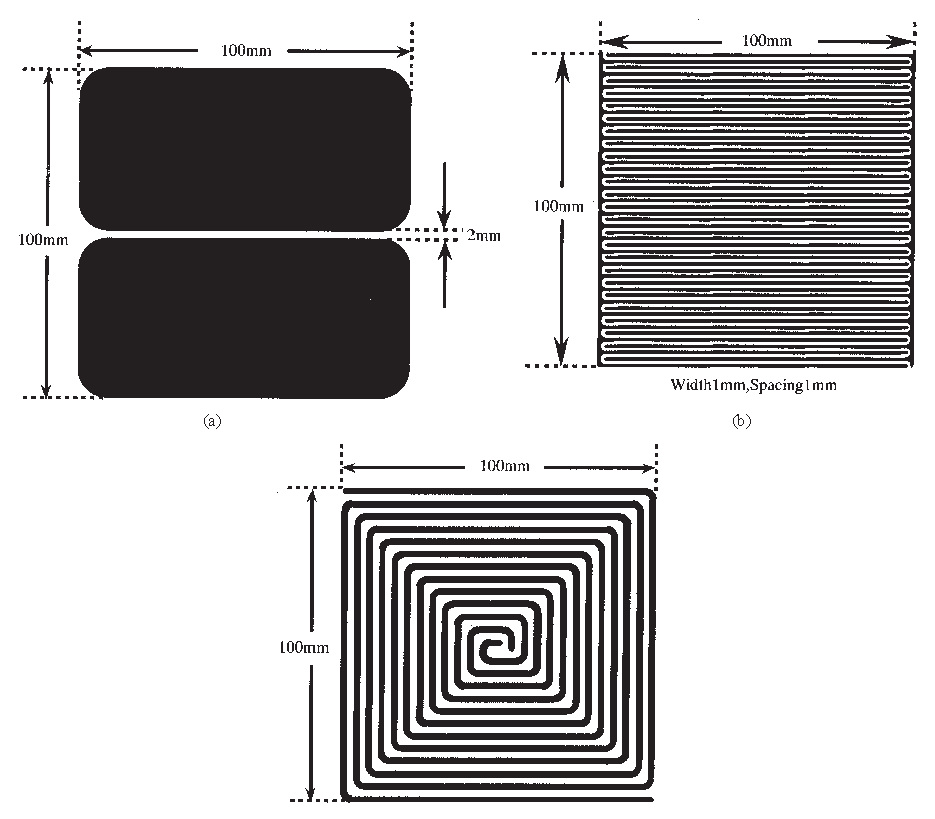
\includegraphics[width=0.7\linewidth]{_a/asano__1}
\caption*{图~A -- 6\hspace{1em}电极布置\quad (a)共平面型\quad (b)\ 平行交错\quad (c)\ 螺旋交错}
\end{figure}

\begin{figure}[tbhp]
\centering
\includegraphics[width=0.7\linewidth]{_a/asano__2}
\caption*{图~A -- 7\hspace{1em}测量系统}
\end{figure}

\begin{figure}[tbhp]
\centering
\includegraphics[width=0.7\linewidth]{_a/asano__3}
\caption*{图~A -- 8\hspace{1em}测力系统\quad (a)横向阻力\quad (b)\ 纵向吸引力}
\end{figure}

\begin{figure}[tbhp]
\centering
\includegraphics[width=0.7\linewidth]{_a/asano__4}
\caption*{图~A -- 9\hspace{1em}不同电极布置与牵引方向对力与电压关系的影响}
\end{figure}

\begin{figure}[tbhp]
\centering
\includegraphics[width=0.7\linewidth]{_a/asano__5}
\caption*{图~A -- 10\hspace{1em}随电极间距的变化关系:\quad (a)\ 力\quad (b)\ 电流}
\end{figure}

\begin{figure}[tbhp]
\centering
\includegraphics[width=0.7\linewidth]{_a/asano__5}
\caption*{图~A -- 10\hspace{1em}随电极间距的变化关系:\quad (a)\ 力\quad (b)\ 电流}
\end{figure}

\begin{figure}[tbhp]
\centering
\includegraphics[width=0.7\linewidth]{_a/asano__6}
\caption*{图~A -- 11\hspace{1em} 横向阻力随电压与绝缘薄膜厚度关系}
\end{figure}

我们测试了很多电极布置,其中部分如\appfigref{A}{6}:\appfigref{A}{6(a)}为共平面电极,下文简称A型;(b)与(c)为不同形状的交错电极,使用印刷电路板(PCB)工艺制成,下文分别简称B、C型。由于我们希望研究静电卡盘的基本特性,试验在大气条件下进行\footnotemark{}。在前期试验中,我们用一张透明幻灯片代替硅晶圆。当使用一张4英寸的硅晶圆做实验时,在晶圆与电极之间插入另一种塑料薄片,用于调节晶圆与电极之间的距离。

\footnotetext{译者注:逻辑不明但原文如此。}

测量系统如\appfigref{A}{7},可切换接通直流或交流电压,其中交流电压包括固定的\SI{50}{\Hz}以及由函数发生器经电压放大器产生的变频交流电压。静电吸引力由\appfigref{A}{8}所示系统测出。靠直接横向牵引晶圆或幻灯片可测出横向阻力,如\appfigref{A}{8(a)};在晶圆上方设置真空吸盘,用绳子通过滑轮,使用直线电机牵引,中间放置应变式力传感器,以此检测竖直方向静电吸引力。

为了探明电极方向性,我们首先横向牵引一张幻灯片。由于幻灯片的材料为PET(聚对苯二甲酸乙二酯),电极上并未覆盖额外的绝缘材料。试验中使用了不同形状参数的电极,如线宽和间距从\SI{0.5}{\mm}变化到\SI{3.0}{\mm}的B型电极。

\appfigref{A}{9}为横向阻力与电压关系,其中电极线宽与间距均为\SI{2}{\mm} mm。双共平面电极(A型)产生的阻力最小;当垂直于B型电极方向牵引时产生的阻力最大,当平行于电极方向时产生的阻力极其微弱;C型电极在各方向产生的阻力基本相等。B型电极显现出的方向性无法用简单的静电理论解释。由于B型电极产生的力高于其他两种,我们选择它作为进一步试验的对象。阻力与电极间距的关系如\appfigref{A}{10}.显然,间距越小,产生力越大;但当间距缩小至\SI{0.5}{\mm}时,试验结果并不理想,这可能是受到电极制造工艺的限制。因此,我们将间距与宽度均为\SI{1}{\mm}的B型电极选为试验基准。

由\appfigref{A}{10(b)}可看出,当电压增加至击穿时,电流迅速增加,为了防止击穿,增加静电吸引力,在电极上喷涂一层绝缘涂料(光刻胶GR-303);使用电容法测量其厚度为约\SI{8}{\um}。之后,又测量了阻力与喷涂的绝缘层厚度的关系,如\appfigref{A}{11};可看出绝缘层越薄,力越强。

\begin{figure}[tbhp]
\centering
\includegraphics[width=0.7\linewidth]{_a/asano__7}
\caption*{图~A -- 12\hspace{1em} 随PE薄膜厚度变化关系:\quad (a)\ 横向阻力\quad (b)\ 电流}
\end{figure}

\begin{figure}[tbhp]
\centering
\includegraphics[width=0.7\linewidth]{_a/asano__8}
\caption*{图~A -- 13\hspace{1em} 残余静电力}
\end{figure}

\begin{figure}[tbhp]
\centering
\includegraphics[width=0.7\linewidth]{_a/asano__9}
\caption*{图~A -- 14\hspace{1em} AC/DC电源对比:\quad (a)\ 力随电压变化\quad (b)\ 电流随电压变化}
\end{figure}

\begin{figure}[tbhp]
\centering
\includegraphics[width=0.7\linewidth]{_a/asano__10}
\caption*{图~A -- 15\hspace{1em} 残余静电力与电流随频率变化关系}
\end{figure}


虽然我们将多种不同材料的绝缘层放置在电极和晶圆中间测试,其中只有PE(聚乙烯)薄膜有多种厚度,因此,大量实验中使用了不同厚度的PE薄膜。由于电极是用PCB工艺刻蚀而成,在电极间存在\SI{35}{\um}高的凸台,导致在施加高压时击穿产生的气隙。因此我们使用硅胶填充这一空隙。横向阻力随电压关系如\appfigref{A}{12}。可见,当PE绝缘层厚度为\SI{50}{\um}高时,可以产生相当强的阻力;当使用更薄的绝缘层时,其表面稳定性变差,经常随晶圆一起被拖动,导致阻力降低。

在使用直流电压试验时,发现残余电荷对试验有很大影响:切断电源较长时间后仍存留有横向阻力。\appfigref{A}{13}是一次测量的结果:初始阻力为\SI{9}{\N}(电压3 kV,绝缘层厚度\SI{50}{\um}),而切断电源12小时后,仍有\SI{4}{\N}阻力残留。为了解决此问题,我们尝试使用高压交流电源。当使用\SI{50}{\Hz}交流电源时,能够消除残余阻力\footnotemark{},但因为电容反复充放电,产生较大反应电流。因此,我们使用函数发生器和电流放大器产生低频高压交流电压。\appfigref{A}{14}比较了使用直流、\SI{1}{\Hz}、\SI{10}{\Hz}电源时产生的阻力和电流大小。如\appfigref{A}{15}所示,采用低频交流供电时,残余阻力大大减小。

\footnotetext{译者注:原文中此处逻辑混乱,疑似为日文直译造成。}

\begin{figure}[tbhp]
\centering
\includegraphics[width=1\linewidth]{_a/asano__11}
\caption*{图~A -- 16\hspace{1em}  静电吸引力随直流电压变化关系:%
\quad (a)\ 介电层厚\SI{16}{\um}%
\quad (b)\ 介电层厚\SI{23}{\um}%
\quad (c)\ 介电层厚\SI{50}{\um}%
}
\end{figure}

为了测量竖直方向上的静电吸引力,使用真空吸盘来夹持晶圆;试验中需确保真空吸盘与晶圆对中。尽管采取了这样的措施,测得的吸引力散布相当大,因此对多组数据取平均值分析。如\appfigref{A}{16},测量了不同电压、不同绝缘层厚度下的吸引力大小,并在图中表示出了平均值。发现静电吸引力较强\footnotemark{}。残余吸引力仍存在,同样可用变频交流供电法消除。

\footnotetext{译者注:原文如此。}

从初期试验中可看出,交错电极型静电卡盘能在塑料薄膜上产生较大的横向阻力,且该阻力随电极间隙减小而增强。然而由于漏电流和击穿强度等因素影响,可能存在一个最优的间隙大小,在我们的试验中得出该大小为\SI{1}{\mm};该值可能与电极制造工艺有关。
当使用\SI{1}{\mm}间隙的电极时,可以在晶圆上产生大于\SI{15}{\N}的静电吸引力。通过改变绝缘层材料与厚度,可以进一步增强静电吸引力。
当电极间存在绝缘材料(包括硅胶)时,即使切断电源,仍存在残余电荷,进而产生残余静电力;可用施加变频交流电压的方式减小这一影响。

\appcite{[1] ASANO K., HATAKEYAMA F., YATSUZUKA K. Fundamental study of an electrostatic chuck for silicon wafer handling[J]. Industry Applications, IEEE Transactions on, 2002, 38(3): 840-845.}
\end{appendix}

% 个人简历
\begin{resume}

	\resumeitem{个人简历}
	
	1991 年 10 月 11 日出生于 黑龙江 省 牡丹江 市。
	
	2010 年 9 月考入 清华 大学 机械工程 系 机械工程及自动化 专业 攻读 工学学士 学位至今。
	
	\begin{comment}
		\resumeitem{发表的学术论文} % 发表的和录用的合在一起
	
		\begin{enumerate}[{[}1{]}]
		\end{enumerate}

		\resumeitem{研究成果} % 有就写,没有就删除
		\begin{enumerate}[{[}1{]}]
		\item 任天令, 杨轶, 朱一平, 等. 硅基铁电微声学传感器畴极化区域控制和电极连接的
		方法: 中国, CN1602118A. (中国专利公开号.)
		\item Ren T L, Yang Y, Zhu Y P, et al. Piezoelectric micro acoustic sensor
		based on ferroelectric materials: USA, No.11/215, 102. (美国发明专利申请号.)
		\end{enumerate}
	\end{comment}
\end{resume}

\end{document}
